\documentclass[11pt]{article}


\title{Federated Truth Discovery for Mobile Crowdsensing with Privacy-Preserving Trustworthiness Assessment}

\author{Leye Wang$^{1,2}$, Guanghong Fan$^{1,2}$, Xiao Han$^{3,}$\footnote{Corresponding author} \\
 \small $^1$Key Lab of High Confidence Software Technologies (Peking University), Ministry of Education, China \\
\small$^2$School of Computer Science, Peking University, China\\
\small$^3$School of Information Management and Engineering, Shanghai University of Finance and Economics, China\\
\texttt{\small leyewang@pku.edu.cn, fgh@stu.pku.edu.cn, xiaohan@mail.shufe.edu.cn}
}

\begin{document}
	
\maketitle

\begin{abstract}
With the prevalence of smart mobile devices empowered by considerable sensing capabilities, crowdsensing has become one promising way to sense urban phenomena (e.g., traffic and environment) at a large scale. In crowdsensing, a fundamental issue is discovering the truth from participants' noisy sensed data. Traditionally, participants need to upload their raw sensed data with locations for truth discovery, but this may leak participants' private information such as home and work locations. In this paper, we propose a federated truth discovery method that can learn the truth without collecting participants' sensed data and locations. Our method ensures that the obtained truth quality has no performance loss compared to the original truth discovery method if all the participants keep online; even if some participants lose connections unpredictably, our method can still learn the truth based on rest participants' data.
Meanwhile, as participants' sensed data are unknown to the server, it is hard for the crowdsensing organizer to justify each participant's sensing trustworthiness. This brings difficulties to crowdsensing management such as participant recruitment and incentive allocation. We further propose a federated ranking mechanism to generate a leader-board for participants' trustworthiness, which can also tolerate participants' connection loss. Both theoretical analysis and real-data empirical evaluations have been done to verify the effectiveness of FedTruthFinder.

\end{abstract}


\section{Introduction}  
\label{s:intro}
The past decade has observed a surge in the design and deployment of 
decentralized systems. A key reason for this surge is the growing desire in 
the society to have self-governing democratic financial systems that are not 
under the control of a privileged set of entities. A central control often 
translates to a forced trust model with limited provision to support 
transparency and accountability. The adoption of Blockchain, for example, 
is a by-product of the ability to break away from the forced-central control 
in a trust-worthy fashion~\cite{blockchain-book}. The emerging blockchain 
platforms facilitate a reliable execution of any digital contracts 
(i.e., transactions) in a decentralized manner despite the existence of malicious 
actors. At the core of any blockchain platform is a Byzantine 
fault-tolerant (\BFT{}) consensus protocol and a tamper-proof replicated 
ledger~\cite{bedrock,blockchain-book,scalable-ledger}. The \BFT{} 
protocol helps to achieve {\em consensus} on the order of incoming client 
requests among all the replicas, while the ledger logs this agreement. 

Traditional \BFT{} protocols expect a {\em permissioned} system where the 
identities of all the replicas (i.e., participants) are known prior to any 
consensus as they rely on having a verifiable voting right in a democratic 
setting. These protocols rely on a {\em communication-oriented} consensus 
model, where all the participants exchange endorsements across multiple 
rounds before they can reach a decision~\cite{sharper,pbftj,ahl,poe,rcc,geobft,flexitrust,ringbft,mirbft,basil,hotstuff}.
In these protocols, a system of $\n{}$ replicas can reach a common decision 
if at most $\f{}$ of them are malicious, such that $\n{} \ge 3\f{}+1$. 
The $\n{}$ parties are said to reach a decision when at least a majority 
of honest parties agrees to that decision. This decision is logged by 
requiring all the agreeing parties to {\em sign} the decision. Hence, the 
reached decision is considered {\em tamper-proof} because it has support 
of a majority of honest participants.

Despite being around for more than two decades, traditional \BFT{} protocols 
did not see any major practical applications until the introduction of 
blockchain technology. We attribute {\em two} key factors for this lack of 
adoption. (i) To ensure that the malicious participants do not spawn multiple 
identities, these \BFT{} protocols need an authority (i.e., {\em a forced 
trust gateway}) to verify and register every participant to verify every 
vote~\cite{sybil-attack}; some participants may find this intrusive if they 
do not want to reveal their personal information. (ii) To overwrite the ledger, 
malicious participants just require access to the private keys of honest 
participants. In a sense, the proof of the validity of the ledger is not 
self-contained, and it operates on the assumption that the private-keys 
are kept safe externally indefinitely.

To resolve these challenges, initial blockchain platforms such as 
Bitcoin~\cite{bitcoin} and Ethereum~\cite{ether} offer a {\em permissionless} 
model of consensus. These systems employ the {\em Proof-of-Work} (\PoW{}) 
protocol~\cite{bitcoin,ether}, which follows a {\em computation-oriented} 
consensus model and requires all the participants to compete with each other 
and try to solve a complex puzzle. Whichever participant solves the puzzle 
first gets to add a new entry ({\em block}) to the ledger. As a result, 
\PoW{} protocol eliminates the three challenges seen by traditional \BFT{} 
protocols. (i) Malicious participants can spawn multiple identities, but what 
actually matters is the available compute power. (ii) Each block includes 
the hash of the previous block; overwriting the ledger requires recomputing 
all the blocks making it computationally infeasible. (iii) Since reaching the 
consensus is based on presenting the proof of work that is embedded on the 
ledger (i.e., self-contained), there is no longer any need for external 
safe-keeping of private keys to sign endorsements.

These properties offered by \PoW{} protocol help blockchain platforms to 
design a {\em decentralized economy}, where any person can participate in the 
consensus process, and the economy has a self-generating currency to monetize 
its participants. Monetizing the participants is necessary as the \PoW{} 
protocol expects the participants to spend their resources to solve a complex 
puzzle. Clients of the Bitcoin platform, create transactions that exchange 
Bitcoins and send them to the participants (miners) in the \PoW{} protocol. 
These miners check if the transaction is valid; the client has sufficient 
Bitcoins to transfer. If the transaction is valid, they run \PoW{} protocol to include 
this transaction in the ledger. The winning miner of \PoW{} gets a portion of 
the client's Bitcoin as {\em fees}, while the mining process (\PoW{}) mints  
new tokens to fund the economy. This new token is transferred to the winning 
miner's account and is recorded as a transaction in the block.

The key challenge with platforms like Bitcoin is their {\em practicality}. 
These platforms have abysmally low throughput in the order of $10$ transactions 
per second in part due to inadequate choice of small block sizes. Furthermore, as 
more miners join the network, the complexity of the puzzle has to be increased. 
For example, the complexity of the current Bitcoin puzzle is so high that the 
miners work in large groups to have any positive probability of creating the 
next winning block~\cite{blockchain-book}. Moreover, as miners are competing 
with each other, it leads to massive wastage of computational resources (energy) 
as only the winning miner's efforts are recorded and rewarded. This results in an unsustainable ecosystem~\cite{badcoin,badbadcoin}.

We observe these challenges in the designs of existing \BFT{} protocols and 
blockchain platforms and envision a \DualChain{} system that learns from these 
models and eliminates their key challenges. Essentially, we aim to establish a 
new research agenda; a new field of hybrid consensus protocols that depart from 
competitive consensus to a collaborative consensus that is both resilient and 
sustainable. Our \DualChain{} architecture takes a step in this direction by 
running two consensuses on each client transaction while ensuring there is no 
increase in the latency observed by the client. Each client request is first 
ordered through a state-of-the-art \BFT{} consensus protocol ({\em commitment}), 
subsequently, this ordered request is engraved into the ledger through the 
\PoW-style consensus ({\em settlement}). Specifically, \DualChain{} causes no 
increase in commitment latency while improving the settlement latency observed 
by existing protocols. Ordering the client transaction through a \BFT{} consensus 
protocol first allows our \DualChain{} system to guarantee the following benefits: 
(i) clients receive low-latency responses, and (ii) \PoW{} participants no longer 
need to compete, resulting in a high-throughput sustainable chain. As a result, 
instead of employing the \PoW{} for consensus, we design a novel protocol that 
allows miners to collaborate. We refer to this paradigm as 
{\em Power-of-Collaboration} (\PoC{}). 

Our \PoC{} protocol splits the complex puzzle into disjoint slices and requires 
each miner to work on a distinct slice. This slice distribution significantly 
reduces the resource wastage and provides each honest miner with a reward 
for each new transaction added to the ledger. As each ledger entry is added 
collaboratively, any malicious entity that wishes to overwrite the ledger 
needs to match the computational power of all the existing miners making it 
practically impossible. These features of our \DualChain{} system make it 
lucrative; its design is the bedrock for a secure and efficient decentralized 
economy.

\section{Preliminary: Truth Discovery}
\label{sec:preliminary}

\begin{figure}
	\centering
	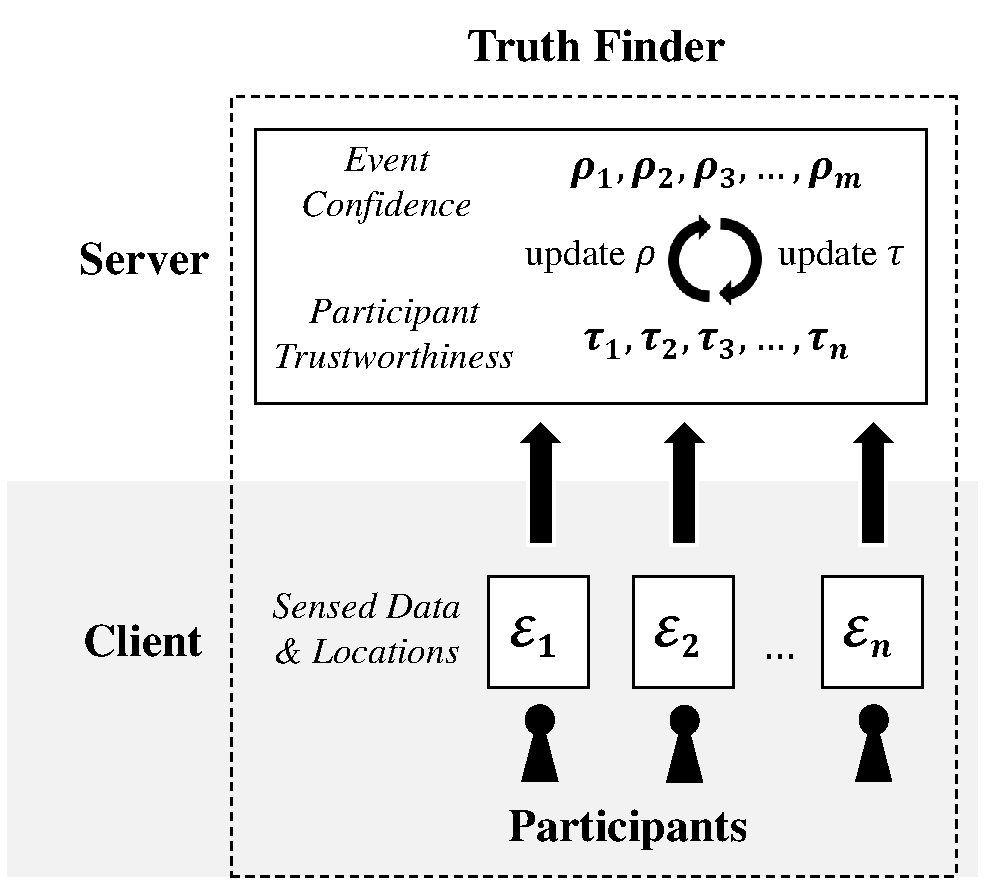
\includegraphics[width=.5\linewidth]{./fig/truthfinder.pdf}
	\caption{Overview of Iterative Truth Discovery}
	\label{fig:truthfinder}
	\vspace{-1em}
\end{figure}


Truth discovery algorithms usually follow an iterative method to calibrate user trustworthiness and data confidence alternatively until convergence \citep{yin2008truth}. Figure~\ref{fig:truthfinder} shows the framework of iterative truth discovery methods. In this paper, for clarity, we assume that sensed data is a binary spatial event. That is, for a specific location, the sensed data can be 1 or 0. Our method can be easily extended to multi-class and continuous-value events (see Appendix). 

As shown in Figure~\ref{fig:truthfinder}, first, participants upload all of their sensed data and locations $\mathcal E_i$  to the central server. The central server would assign an initial trustworthiness score $\tau_i$ to each participant $u_i$ (e.g., 0.9 by assuming that 90\% of the sensed data are accurate). Then, for each sensed event $e_j$, the truth discovery algorithm will calculate its confidence $\rho_j$ (i.e., the probability of $e_j = 1$) by considering the users who have sensed $e_j$ as:
\begin{equation}
\rho_j = F_\rho(\mathcal U_{j,1}, \mathcal U_{j,0})
\label{eq:event_confidence}
\end{equation}
where $\mathcal U_{j,k}$ is the users who have sensed the event $e_j$ with the reported data $k$; $F_\rho$ is an event confidence calculation function which we will elaborate on later. 

With $\rho_j$ for each event $e_j$, we can then update the trustworthiness score $\tau_i$ of each participant $u_i$ by:
\begin{equation}
\tau_i = F_\tau(\mathcal E_{i,1}, \mathcal E_{i,0})
\end{equation}
where $\mathcal E_{i,k}$ is the users' sensed event set with the reported data $k$; $F_\tau$ is a user trustworthiness calculation function which we will elaborate on later. 

Once $\tau_i$ is updated for each user $u_i$, we can continue updating $\rho_j$ for each event $e_j$ according to Eq.~\ref{eq:event_confidence}, and so on, leading to an alternative updating process for both $\tau_i$ and $\rho_j$. This process can be terminated after a fixed number of iterations or until convergence. Next, we elaborate on the common choices of $F_\rho$ and $F_\tau$ in literature.

\textbf{Sum Function}

An intuitive selection of the updating functions of $F_\rho$ and $F_\tau$ is the weighted sum:
\begin{equation}
\rho_j = F_\rho(\mathcal U_{j,1}, \mathcal U_{j,0}) = \frac{\sum_{u_i \in \mathcal U_{j,1}} \tau_i}{\sum_{u_i \in \mathcal U_{j,1}} \tau_i + \sum_{u_k \in \mathcal U_{j,0}} \tau_k}
\label{eq:rho_function_sum}
\end{equation}
\begin{equation}
\tau_i = F_\tau(\mathcal E_{i,1}, \mathcal E_{i,0}) = \frac{\sum_{e_j \in \mathcal E_{i,1}} \rho_j + \sum_{e_k \in \mathcal E_{i,0}} 1-\rho_k}{|\mathcal E_{i,1}|+|\mathcal E_{i,0}|}
\label{eq:tau_function}
\end{equation}

\textbf{Logistic Function}

Another widely used updating function is the Logistic function \citep{yin2008truth}. Its basic idea is seeing every user independently, so that the probability of event happening, i.e., $e_j=1$, can be formulated as:
\begin{equation}
	\rho_j = 1 - \prod_{u_i \in \mathcal U_{j,1}} (1-\tau_i)
\end{equation}
As $1-\tau_i$ may often be small and multiplying many of them may lead to underflow, prior studies proposed to use the logarithm to define a log-trustworthiness score of $u_i$ as \citep{yin2008truth}:
\begin{equation}
	\tau_i^* = - \ln(1-\tau_i)
\end{equation}
Similarly, a log-confidence score of event $e_j$ is defined as:
\begin{equation}
	\rho_j^* = - \ln(1-\rho_i)
\end{equation}
Then, we can infer 
\begin{equation}
	\rho_j^* = \sum_{u_i \in \mathcal U_{j,1}} \tau_i^*
\end{equation}
The above equation does not consider the users' trustworthiness who report $e_j=0$, and thus we refine it:
\begin{equation}
	\rho_j^* = \sum_{u_i \in \mathcal U_{j,1}} \tau_i^* - \sum_{u_k \in \mathcal U_{j,0}} \tau_k^*
\end{equation}
Finally, a logistic function is used to calculate the final confidence $\rho_j$ of event $e_j$ \citep{yin2008truth}:
\begin{equation}
	\rho_j = F_\rho(\mathcal U_{j,1}, \mathcal U_{j,0}) = (1+e^{-\rho_j^*})^{-1}
	\label{eq:rho_function_log}
\end{equation}
$\tau_i$ is updated same as Eq.~\ref{eq:tau_function}.
\section{Method}

Here we discuss the standard retrieve-and-rerank (R\&R) framework for IR (\S{\ref{sec:retrieve_and_rerank}}) and how our proposal fits into it (\S{\ref{sec:cross_encoder_feedback}}). While our approach can be applied to any R\&R framework, we consider a text-based retriever and reranker for simplicity while elaborating our method. A multi-modal R\&R framework is described in \S\ref{sec:multimodal_results}.


\subsection{Retrieve-and-Rerank}
\label{sec:retrieve_and_rerank}
R\&R for IR consists of a first-stage retriever and a second-stage reranker. Modern neural approaches typically use a dual-encoder model as the retriever and a cross-encoder for reranking.  

\paragraph{\textbf{The Retriever}:} The dual-encoder retriever model is based on a Siamese neural network \cite{chicco2021siamese}, containing separate Bert-based \cite{devlin2019bert} encoders $E_Q(.)$ and $E_P(.)$ for the query and the passage, respectively.
Given a query $q$ and a passage $p$, a separate representation is obtained for each, such as the \textsc{cls} output or a pooled representation of the individual token outputs from $E_Q(q)$ and $E_P(p)$. The question-passage similarity $sim(q,p)$ is computed as the dot product of their corresponding representations: query/passage.}
\begin{equation}
    Q_q = Pool(E_Q(q))
\end{equation}
\begin{equation}
    P_p = Pool(E_P(p))
\end{equation}
\begin{equation}\label{eq:sim}
   sim(q,p) = S(Q_q,P_p) = Q_q^TP_p
\end{equation}

Since Eq.~\ref{eq:sim} is decomposable, the representations of all passages in the retrieval corpus can be pre-computed and stored in a dense index \cite{johnson2019billion}. During inference, given a new query, the top $K$ most relevant passages are retrieved from the index via approximate nearest-neighbor search.

\paragraph{\textbf{The Reranker}:} The cross-encoder reranker model uses a Bert-based encoder $E_R(.)$, which takes the query $q$ and a corresponding retrieved passage $p$ together as input and outputs a similarity score. 
A feed-forward layer $F$ is used on top of the \textsc{cls} output from $E_R(.)$ to compute a single logit, which is used as the final reranker score $R(q,p)$. The top $K$ retrieved passages are then ranked based on their corresponding reranker scores.

\begin{equation}
   R(q,p) = F(CLS(E_R(q,p))
\end{equation}


\begin{algorithm}[t]
\caption{\textsc{\textbf{ReFIT}}}
\label{alg4}
\begin{flushleft}
\textbf{Input}: Query $q$ and its representation $Q_q$, retrieved passages $P$ and their representations $\hat{P}$.\newline
\textbf{Output}: Updated query representation $Q_{q,n}$
\end{flushleft}
\begin{algorithmic}[1]
    \State Initialize query vector $Q_{q,0}$ = $Q_q$
    \State Compute reranker distribution $D_{CE}(q,P)$ (Eq.~\ref{eq:d-ce})
    \For{\textit{i in 0 to n}}
        \State Compute retriever distribution $D_{Q_{q,i}}(\hat{P})$ (Eq.~\ref{eq:d-q})
        \State Compute loss $\mathcal{L}$ (Eq.~\ref{eq:loss})
        \State Update $Q_{q,i+1} = Q_{q,i} - \alpha \frac{\partial}{\partial Q_{q,i}}\mathcal{L}$
    \EndFor
    \State return $Q_{q,n}$
\end{algorithmic}
%\vspace{-0.4em}
\end{algorithm}

\subsection{Reranker Relevance Feedback}
\label{sec:cross_encoder_feedback}
The main idea underlying our proposal is to compute an improved query representation for the retriever using feedback from the more powerful reranker.
More specifically, we perform a lightweight inference-time distillation of the reranker's knowledge into a new query vector.

Given an input query $q$ during inference, we use the following output provided by the R\&R pipeline:
\begin{itemize}
   \item Query representation $Q_q$ from the retriever.
    \item Retrieved passages $P = \{p_1, p_2,  ..., p_K\}$ and their representations $\hat{P} = [P_{p_1}, P_{p_1},  ..., P_{p_K}]$ from the retriever. 
    \item The reranking scores $R(q,P) = [R(q,p_1),..., R(q,p_K)]$.
\end{itemize}
Note that $\hat{P}$ above is directly obtained from the passage index and is not computed during inference.

The proposed reranker feedback mechanism begins with using the reranking scores $R(q,P)$ to compute a cross-encoder ranking distribution $D_{CE}(q,P)$ over passages $P$ as follows:

\begin{equation}
D_{CE}(q,P)=\mathrm{softmax}([R(q,p_1), ..., R(q,p_K)])
\label{eq:d-ce}
\end{equation} 

The query and passage representations from the retriever are used to compute a similar distribution $D_{Q_q}(\hat{P})$ over $P$:

\begin{equation}
    D_{Q_q}(\hat{P}) = \mathrm{softmax}([Q_q^TP_{p_1}, ..., Q_q^TP_{p_K}])
    \label{eq:d-q}
\end{equation}

Next, we compute the loss as the KL-divergence between the retriever and reranker distributions:

\begin{equation}
    \mathcal{L} = D_{KL}(D_{CE}(q,P) || D_{Q_q}(\hat{P}))
    \label{eq:loss}
\end{equation}

which is then used to update the query vector via gradient descent. The query vector update process is repeated for $n$ times, where $n$ is a hyper-parameter. 
A schematic description of the process can be found in Algorithm \ref{alg4}. 

Finally, the updated query vector $Q_{q,n}$ is used for a second-stage retrieval from the passage index.  
From dual-encoder retrieval with the updated $Q_{q,n}$, we aim to achieve better recall than with the initial $Q_q$, while obtaining a ranking performance that is comparable with that of the reranker.







\section{Federated Trustworthiness Rank}
\label{sec:trust_ranking}

While FedTruthFinder learns the integrated event truth in a privacy-preserving manner, it brings a challenge in justifying participants' trustworthiness. For example, to incentivize the crowdsensing participants, it is a common strategy to pay the high-trustworthy participants (i.e., high-quality sensing results) with higher incentives. However, in FedTruthFinder, the sensing quality of each participant, i.e., the trustworthiness score $\tau_i$ is kept at each participant side and unknown to the server. Hence, how to assess participants' trustworthiness is required and challenging for FedTruthFinder.

In this section, we first illustrate a concrete case to describe that $\tau_i$ cannot be directly known to the server, otherwise the server may infer which event $u_i$ has sensed. As $\tau_i$ cannot be known to the server, we then design a secure ranking algorithm to let the server know every participant $u_i$'s ranking position of $\tau_i$ among all the participants without leaking $\tau_i$. Based on the ranked positions, the crowdsensing organizer can enable certain trustworthiness-aware incentive mechanisms, e.g., rewarding high-position participants with bonus, which can incentivize participants to compete with each other to get more high-quality sensed data \citep{Reddy2010ExaminingMF}.

\subsection{Privacy Leakage by Trustworthiness $\tau_i$}

Here, we illustrate an example to show the risk of revealing $\tau_i$ to the server for leaking participant $u_i$'s privacy.

Without the loss of generality, we assume that $u_1$'s $\tau_1 = 0.9$, and other $u_i$'s $\tau_i < 0.9\ (i\not=1)$. Suppose that one event $e_j$'s $\rho_j = 0.9$ after truth discovery, then we can easily infer that $u_1$ has sensed the event $e_j$ and the sensed result is $1$. This reveals the fact that $u_1$ has visited the location of $e_j$, leaking $u_1$'s location privacy.

Hence, participants cannot directly upload their $\tau_i$ to the server for incentive allocation. Next, we design a privacy-preserving method to enable trustworthiness-aware incentive allocation. 

\subsection{Secure Trustworthiness Leader-board}

While revealing $\tau_i$ may leak participants' private information, we propose a secure ranking algorithm to learn a  leader-board regarding participants' trustworthiness for facilitating trustworthiness-aware incentive allocation.

Secure ranking algorithms have been studied for decades; however, prior studies cannot be directly applied in our scenario for two reasons. First, the communication overheads are usually high. Second, prior studies mostly assume that all the network connections are stable for all the parties, but this is unrealistic for crowdsensing. 

Our secure ranking algorithm generally follows the design of \citet{tang2011secure}. However, the original design \citep{tang2011secure} cannot tolerate any participants to lose the network connections. We thus enhance it to ensure that the ranking algorithm can still work when certain participants lose connections.
The major steps of our federated trustworthiness leader-board generation mechanism are:

\textbf{Step 1}. First, we categorize all the participants into $(2t+1)$ groups, and thus each group includes $n/(2t+1)$ participants. We denote $gid(u)$ to refer to the group ID of participant $u$.

\textbf{Step 2}. For each user $u_i$, she shares $\tau_i$, $\tau_i^2$, ... , $\tau_i^{2t+1}$ with $(t+1, 2t+1)$-SSS to all the user groups. Specifically, a user $u_j$ will receive the share piece regarding $gid(u_j)$, denoted as $\tau_{i_1}(gid(u_j))$, $\tau_{i_2}(gid(u_j))$, ... $\tau_{i_{2t+1}}(gid(u_j))$ for $\tau_i$, $\tau_i^2$, ... , $\tau_i^{2t+1}$, respectively.

\textbf{Step 3}. For each user group $g_k$, it generates a random number $r_k (>0)$ and shares $r_k$ with $(t+1, 2t+1)$-SSS to all the user groups. That is, $u_j$ will receive $r_k$'s share regarding $gid(u_j)$, denoted as $r_k(gid(u_j))$.

\textbf{Step 4}. For each participant $u_j$, she calculates the following number with the $\tau_{i_k}(gid(u_j))$ received from $u_i$:
\begin{align}
h_{i}(gid(u_j)) &= \lambda(gid(u_j)) \sum_{k=1}^{2t+1} r_k(gid(u_j)) \tau_{i_k}(gid(u_j)) \\ &= \lambda(gid(u_j)) \gamma(gid(u_j))
\end{align}
where
\[
\left(\begin{array}{ccccc} 
	1 &    1 & 1^2 & ...  & 1^{2t} \\ 
	1 &    2 & 2^2 & ... & 2^{2t}\\
	... & ... & ... & ...& ...\\
	1 & 2t+1 & (2t+1)^2 & ... & (2t+1)^{2t}\\
\end{array}\right)^{-1} 
\]
\[
=\left(\begin{array}{ccccc} 
	\lambda(1) &   \lambda(2) & \lambda(3) & ...  & \lambda(2t+1) \\ 
	... & ... & ... & ...& ...\\
	... & ... & ... & ...& ...\\
	... & ... & ... & ...& ...
\end{array}\right) 
\]


\textbf{Step 5}. For each user group, we randomly select one participant $u_j$ to share $\{h_{i}(gid(u_j))| i \in [1,n]\}$ with $(t+1, n)$-SSS to all the $n$ participants. Each user $u_k$'s received shares from all the groups are denoted as $\{h_i(g, k)| i \in [1,n], g \in [1, 2t+1]\}$.

\textbf{Step 6}. For each participant $u_k$, she computes:
\begin{equation}
h'_i(k) = \sum_{g=1}^{2t+1} h_i(g, k), \quad \forall i \in [1,n]
\end{equation}
Each $u_k$ sends $\{h'_i(k)| i\in[1,n]\}$ to the server.

\textbf{Step 7}. After receiving at least $t+1$ participants' $\{h'_i(k)| i\in[1,n]\}$, the server can recover:
\begin{equation}
	h_i = \sum_{k=1}^{2t+1} r_k \tau_i^k, \quad \forall i \in [1,n]
\end{equation}

\textbf{Step 8}. The server ranks $u_i$ according to $h_i$ and the ranked list is the leader-board regarding trustworthiness $\tau_i$.

Note that same as $\rho$-computation, we do not need to establish the peer-to-peer communication channels between every two participant clients and can use the crowdsensing server for coordination. To avoid redundancy, readers can refer to Sec.~\ref{subsub:server_coordination} for details.

\textbf{Remark on our novelty}. The key improvement of our secure ranking algorithm compared to \citet{tang2011secure} is the enhanced robustness against participants' connection loss. In \citet{tang2011secure}, every participant holds a $r_i$ and we will randomly select $2t+1$ participants to share their $r_i$ (Step 3) and $h_i$ (Step 5). This process is easy to break if a selected online user (Step 3) loses the connection in Step 5. Our proposed algorithm first constructs user groups so that we only need at least one participant online in each group for both Step 3 and 5, reducing the failure possibility incurred by connection loss. It is worth noting that this algorithm can not only rank crowdsensing participants' trustworthiness, but also be applied to many other applications when privacy-preserving data ranking is needed under unstable network connections.

\textbf{Remark on the ranked measurements}. In the previous algorithm description, we suppose that $\tau_i$ needs to be ranked. In practice, crowdsensing organizers can use the same secure ranking mechanism to rank other key measurements of participants (e.g., the number of sensed events) to design better incentive mechanisms or participant recruitment strategies.

\subsection{Theoretical Analysis}
\label{sub:theoretical_analysis_2}

All the proofs are illustrated in Appendix.

\subsubsection{Correctness} We first prove the correctness of our algorithm.

\vspace{+.5em}
\textbf{Lemma 5.1}. $\sum_{k=1}^{2t+1} r_k(x)\tau_{i_k}(x)$ can be represented as:
$$h_{i}+a_{i1}x+a_{i2}x^2+...+a_{i2t}x^{2t}$$
where $h_i=\sum_{k=1}^{2t+1} r_k\tau_i^k$. \citep{tang2011secure}
 
\vspace{+.5em}
\textbf{Theorem 5.1}. With $t+1$ participants' $h'_i(k)$, we can recover $h_i$.

\begin{figure*}[t!]%[tbhp]
	\centering
		\begin{subfigure}[t]{.325\linewidth}
			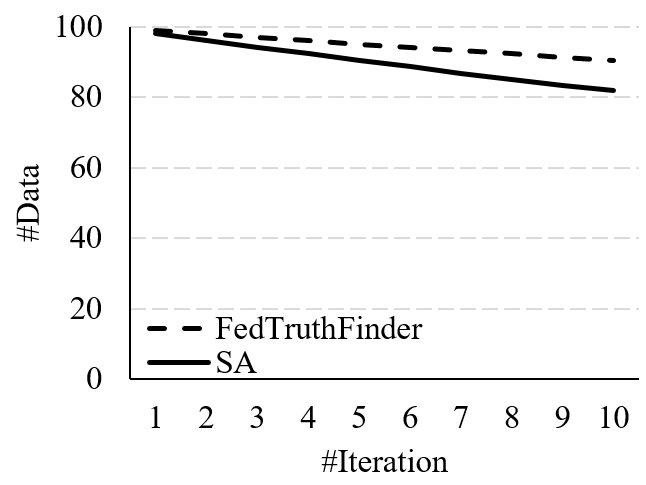
\includegraphics[width=1\linewidth]{./fig/data_num_cl0.01.PNG}
			\caption{$p_l=0.01$}
			\label{fig:cl0.01}
		\end{subfigure}
		\begin{subfigure}[t]{.325\linewidth}
			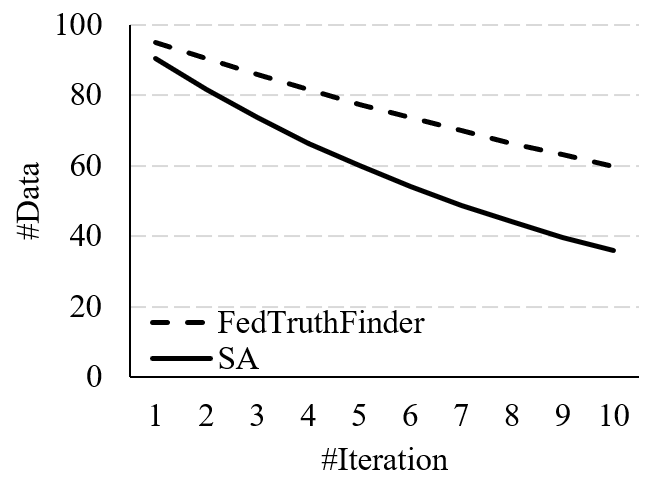
\includegraphics[width=1\linewidth]{./fig/data_num_cl0.05.PNG}
			\caption{$p_l=0.05$}
			\label{fig:chicago}
		\end{subfigure}
		\begin{subfigure}[t]{.325\linewidth}
			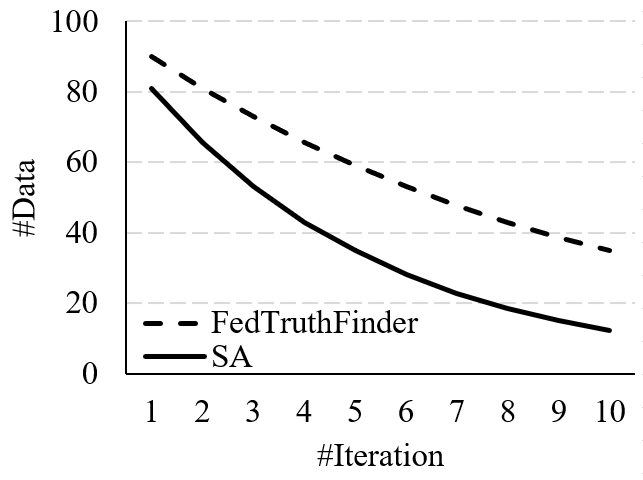
\includegraphics[width=1\linewidth]{./fig/data_num_cl0.1.PNG}
			\caption{$p_l=0.1$}
			\label{fig:dc}
		\end{subfigure}
		\caption{Number of data for each event's truth discovery by iterations.}
		\label{fig:num_sensed_data}
\end{figure*}

\begin{figure*}
	\centering
		\begin{subfigure}[t]{.3\linewidth}
			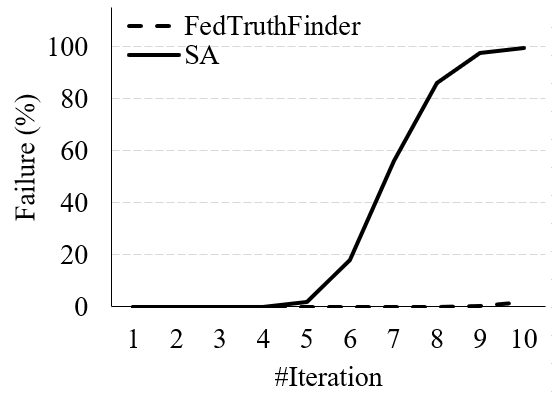
\includegraphics[width=1\linewidth]{./fig/failure_cl0.05.PNG}
			\caption{$p_l=0.05$}
		\end{subfigure}
		\begin{subfigure}[t]{.3\linewidth}
			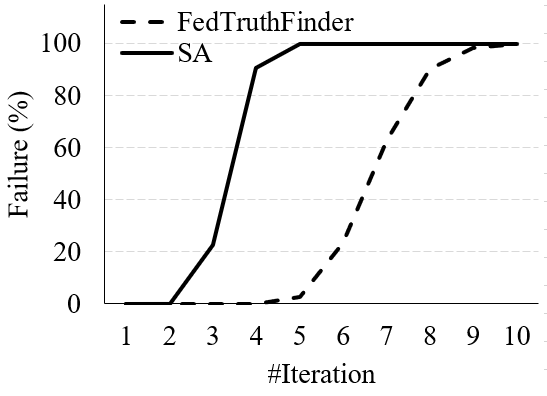
\includegraphics[width=1\linewidth]{./fig/failure_cl0.1.PNG}
			\caption{$p_l=0.1$}
		\end{subfigure}
		\caption{Failure probability of truth discovery.}
		\label{fig:failure}
\end{figure*}

\vspace{+.5em}
\textbf{Theorem 5.2}. Ranking $h_i$ is equivalent to ranking $\tau_i$.


\subsubsection{Robustness to Connection Loss} We analyze how our secure ranking algorithm can tolerate connection losses. We assume that before Step 2, there is no user connection loss.\footnote{If $u_i$ loses the connection in Step 2 and cannot share $\tau_i^k$ with SSS, then there is no way to rank $u_i$'s position because the server has no $u_i$'s information.}

\vspace{+.5em}
\textbf{Theorem 5.3}. To finish Step 3-5, there needs at least one user online for each group. Suppose that every user has $p_l$ probability to lose connection and there are $n$ users, the success probability $\ge (1-p_l^{\lfloor n/(2t+1) \rfloor})^{2t+1}$.


\vspace{+.5em}
\textbf{Theorem 5.4}. To finish Step 6-8, $\ge t+1$ users need to be online.



\subsubsection{Security} Here, we analyze the security of our mechanism.

\vspace{+.5em}
\textbf{Theorem 5.5} If there are no more than $t$ collusive participants, then these participants cannot recover all the other users' $\tau_i$.






\subsubsection{Complexity} We analyze the algorithm from communication and computation complexity perspectives for participant clients.

\textbf{Communication Complexity - $O(tn)$}. In Step 2, the communication overhead of one participant to send $\tau_i,\tau_i^2,...,\tau_i^{2t+1}$ is $O(t^2)$, while each user received data is $O(tn)$. In Step 3, the complexity is $O(t)$. In Step 5, for sending data, the complexity is $O(n)$; for receiving data, the complexity is $O(tn)$. In Step 7, the complexity is $O(n)$. Combing them together, the communication complexity of the whole process is $O(tn)$ as $t<n$.


\textbf{Computation Complexity - $O(tn)$}. The main computation processes of each client include (1) calculating secret shares for $\tau_i,\tau_i^2,...,\tau_i^{2t+1}$ with $(t+1, 2t+1)$-SSS in Step 2, which is $O(t^2)$, (2) calculating secret shares of $r_k$ in Step 3, which is $O(t)$, (3) computing  $h_i$ in Step 4, which is $O(tn)$, and (4) calculating $h_i'$ in Step 6, which is $O(tn)$. Hence, the final computation complexity is $O(tn)$.

\subsection{Experimental Setup}
In this section, we empirically evaluate the effectiveness and interpretability of the proposed~\dname~on both
simulation and real-world datasets.
For interpretability, we focus on whether the algorithm can uncover the causal relationships inherent in the knowledge graph.


\subsubsection{\textbf{Baselines}}
% The aim of this experiment was to evaluate both the effectiveness and interpretability of the existing methods and our approach.
% In this paper, we design a causal rule-based prediction algorithm mainly for application scenarios that require explainability.
To evaluate the interpretability of the algorithms, we select four rule-based methods
that can conduct link prediction and generate explainable rules.
To make a fair comparison, the inference rules, obtained from different algorithms, are used to conduct the link prediction task based on the same prediction equations.
This approach can also help us observe the impact of different rules on the link prediction task.
For a complete evaluation of the effectiveness of the proposed approach, we also compute the LP performance of TuckER\cite{balazevic2019tucker}, one representation-based method which has the best overall performance among the representation-based methods across different datasets\cite{rossi2021knowledge}.
All baselines are listed in the following:
\begin{itemize}
\item[1)] AMIE+\cite{galarraga2015fast}, an efficient  top-down method to discover the interpretable rules.
\item[2)] AnyBURL\cite{meilicke2019anytime}, a bottom-up approach to mine the logical rule.
\item[3)] Neural-LP\cite{yang2017differentiable}, an end-to-end differentiable model to learn the first-order logical rule.
\item[4)] RNNLogic\cite{qu2020rnnlogic}, an EM-based algorithm to learn the rule generator and the reasoning predictor iteratively.
\item[5)] TuckER\cite{balazevic2019tucker},  a linear model based on Tucker
decomposition of the binary tensor representation of knowledge graph triples.
\end{itemize}





\subsubsection{\textbf{Datasets}}
To quantitatively evaluate the effectiveness of the algorithm in discovering causal knowledge, we construct a simulation dataset owing to a lack of groundtruth of real datasets.
Douban and Hetionet~\cite{himmelstein2017systematic} are selected as our real datasets on which we perform two link prediction tasks, movie rating prediction and drug repurposing, respectively.
Here we provide more details for these datasets, and their statistics are shown in Table~\ref{tab:dataset_statistics}.

% \begin{figure}[t]
% \vspace{0cm}
% \centering
% 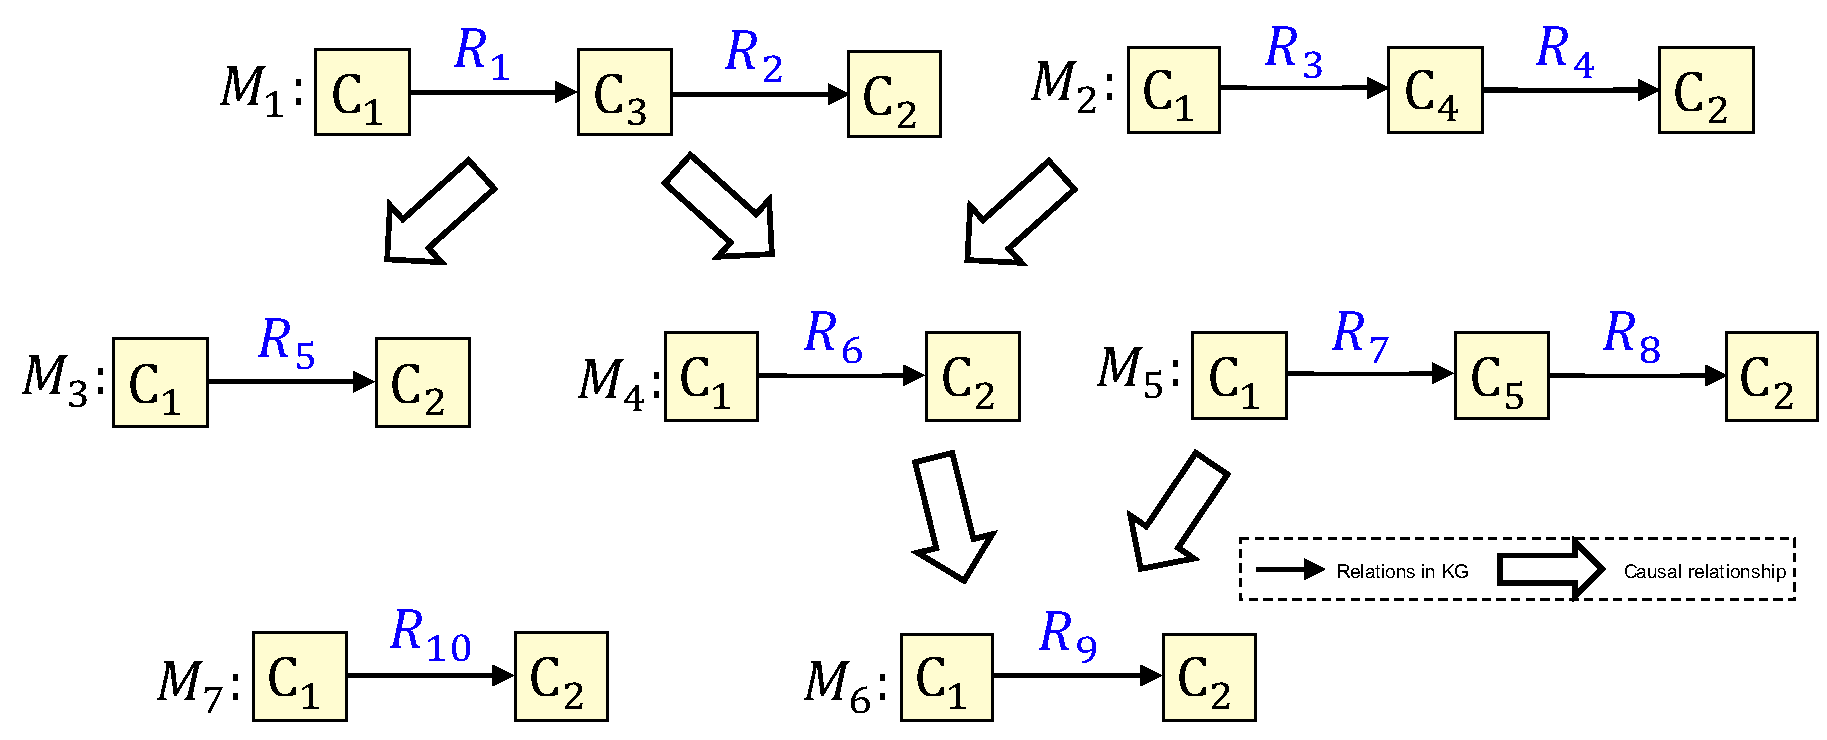
\includegraphics[width=8.5cm]{./figures/simulation.pdf}
% \caption{ The causal graph used to generate simulated knowledge graphs.}
% \label{fig:toy_example}
% \end{figure}

\begin{table}[t]
\centering
\caption{Dataset statistics of all the experiments.}
\label{tab:dataset_statistics}
% \vspace{-2pt}
\scalebox{1}{
\begin{tabular}{c|ccc}
\hline
   & \textbf{\#Triplets} & \textbf{\#Relations} & \textbf{\#Entities}  \\
\hline
\textbf{Simulation} & 6,095 & 5 & 1,590\\
\textbf{Douban Movie Rate} & 28,356 & 12 & 3,007 \\
\textbf{Hetionet} & 174,941 & 20 & 32,056 \\
\hline
\end{tabular}
}
\end{table}

\noindent
{\bf Simulation dataset.}
We generate simulated KGs based on a toy causal model specified in Fig.~\ref{fig:simulation}, which includes three concepts and five relations.
In particular, we design the causal mechanisms in KG via a probabilistic model.
The root nodes ($X_1$, $X_4$) in the causal graph are generated via Bernoulli distributions, whose probability mass function is $f_X(x)=p^x(1-p)^{1-x}$.
Moreover, the non-root nodes ($X_2$, $X_3$) are generated via the conditional probability distributions, which are Bernoulli distributions, given the parent node ($X_1$).
To maintain a stable causal mechanism, the parameters of conditional distributions are constant in training and testing, as shown in Table~\ref{tab:simulation_set}.
In the out-of-distribution paragraph, we will introduce the parameters of root nodes in training and testing.


\begin{figure}[h]
\centering
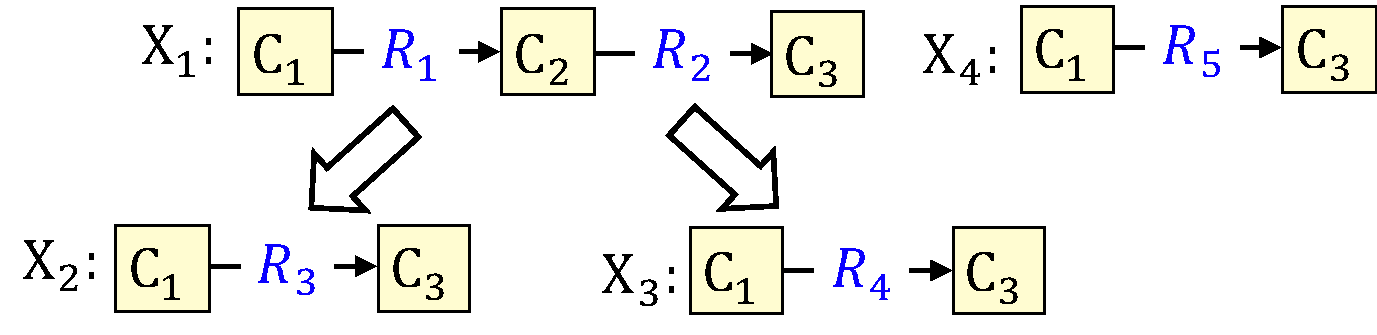
\includegraphics[width=7cm]{submissions/causal-meta-knowledge/figures/simulationv4.pdf}
\caption{The causal graph of relation paths, based on which the simulated KGs are generated .}
\label{fig:simulation}
% \vspace{-2pt}
\end{figure}

\begin{table}[h]
\caption{The parameters of conditional distributions.}
%\vspace{5pt}
\label{tab:simulation_set}
\centering
\scalebox{1}{
\begin{tabular}{c|cccc}
\hline
Conditions & $X_2|X_1=1$ & $X_2|X_1=0$ & $X_3|X_1=1$ & $X_3|X_1=0$ \\
\hline
Parameters & $p$=0.9 & $p$=0.1 & $p$=0.9 & $p$=0.1 \\
\hline
\end{tabular}}
% \vspace{-2pt}
\end{table}
% We generate simulated KGs based on a toy causal model specified in Fig.~\ref{fig:toy_example}, which includes five concepts and ten relations.
% More specifically, given $N$ entities for each concept, the facts containing the relations in the root nodes ($M_1$, $M_2$, $M_7$) of the causal graph are generated via Bernoulli distributions, whose probability mass function is $f(x)=p_r^x(1-p_r)^{1-x}$.
% For example, the entity pair $(e_1,e_3)$, where $e_1 \in \mathcal{E}_{C_1}$ and $e_3 \in \mathcal{E}_{C_3}$, the probability that the fact $<e_1,R_1,e_3> \in \mathcal{G}$ is $p_r$.
% % It means for any entity pair $(e_h,e_t)$, where $e_h \in \mathcal{E}_{C_h},\mathcal{E}_{C_t}$ and $R_i(C_h,C_t) \in \text{KG schema} \mathcal{S}$, the probability that the fact $R_i(e_h,e_t) \in \mathcal{T}$ is $p_r$.
% % we design the conditional  probabilistic distribution in SPRM based on which to sample the entity and facts in KG.
% And the facts in non-root nodes (e.g., $M_3$) are generated via the conditional probability distributions, which are Bernoulli distributions with parameter set $\mathbf{p}_{nr}$, given the facts information of parent node ($M_1$).
% For example, if there is a path instance of $M_1$ between $(e_1,e_3)$, then the probability of the existence of fact $<e_1,R_5,e_3>$ is $p_{M_1=1}$, otherwise is $p_{M_1=0}$.
% \yym{the value of all parameter of $p_nr$}

%


\noindent
{\bf Douban movie rating.}
Douban is a famous Chinese website for movie reviews, where users can rate and comment on any movie.
The rating range is from 1 to 5. A higher rating means that users like movies, while a lower rating means that users have negative feedback on movies.
We collect the real-world data from Douban\footnote{https://www.douban.com/} and construct a dataset (this dataset will be released), whose statistics are shown in Table~\ref{tab:dataset_statistics}.
Commonly, a movie with a score of 4 or 5 is identified as meeting the taste of users.
So we transform the original 5-level rating to a 2-level rating with a threshold of 4.
If the rating score is 4 or 5, the original relation \textit{Rate} is replaced by  \textit{HighRate}
We conduct the link prediction task on the relation \textit{HighRate}.
Because the raw data is too large and the relations between users and movies are very sparse, in this thesis, we first filter the 20 users who have made the most ratings and take the rating history of these users as the set of rating facts for our study.
The facts unrelated to the rating are also included in our experimental data.

\noindent
{\bf Hetionet}\cite{himmelstein2017systematic}
is a freely available knowledge database that integrates biomedical information from 29 prominent
bioinformatics resources.
Recently, Hetionet was successfully applied to drug repurposing tasks in terms of the link prediction task for relation \texttt{Treats}\cite{himmelstein2017systematic, ratajczak2022task}.

\textit{Why do we choose those two real datasets instead of other commonly used datasets, such as WN18, FB15k?}
In this paper, we focus on link prediction with the help of causal relationships between knowledge graph relations.
The core of causality lies in its asymmetry.
The commonly used KGs for link prediction algorithms contain many symmetrical relationships, e,g., \textit{hypernym} and \textit{hyponym} in WN18.
These symmetrical relationships may help with the link prediction task, but they go against the basic idea that causality is a one-way relationship.
We, therefore, chose datasets with specific application scenarios and rich causal semantics.

\subsubsection{\textbf{Metrics.}}
\textbf{For link prediction}, we employ the commonly used metrics mean reciprocal rank (MRR) and Hits@k~\cite{rossi2021knowledge,balazevic2019tucker,bordes2013translating}.
\begin{equation}
\label{eq:mrr}
\begin{aligned}
M R R=\frac{1}{|Q|} \sum_{q \in Q} \frac{1}{q}
\end{aligned}
\end{equation}

\begin{equation}
\label{eq:hitk}
\begin{aligned}
Hit@K=\frac{|\{q \in Q: q \leq K\}|}{|Q|}
\end{aligned}
\end{equation}
where $Q$ is the rank results, for each $q_i \in Q$ is the ranking of the desired results in the $i$-th query $(?,R_h,e_t)$.
In the case of ties in the calculation of $Q$, we use the mean rank to avoid misleading results\cite{rossi2021knowledge,ruffinelli2020you}.
% Common values for $K$ are 1, 3, 5, 10, we use $K=5$ in this paper.
Both MRR and His@k are the higher, the better.

\noindent
\textbf{The interpretability of causal rules} on the simulation dataset can be understood as the consistency between the mined causal rules and the actual causal structure.
Therefore, we evaluate baselines and our approach on the simulation dataset using precision, recall, and structural Hamming distance (SHD) as the evaluation metrics, which are commonly used evaluation metrics in causal structure discovery studies~\cite{zheng2018dags,zheng2020learning}.
% Since the performance of causal rule discovery is the foundation of our link prediction method.

\begin{equation}
\label{eq:precision}
\begin{aligned}
Precision=\frac{\# TFR}{\#FR};Recall=\frac{\# TFR}{\#ATR}
\end{aligned}
\end{equation}
Where $\#TFR$ is the number of right causal relationships discovered by an algorithm, $\#FR$ is the number of causal relationships discovered by an algorithm, and $\#ATR$ is the number of all causal relationships.
Both precision and recall are the higher, the better.
SHD calculates the difference between the learned graph and the ground truth graph by the number of edge insertions, deletions, or flips required to transform one graph into another.
The lower the SHD, the better.

\subsubsection{\textbf{Out-of-Distribution Link Prediction}}
Traditional machine learning methods are designed based on the assumption of independent and identically distributed (I.I.D) data.
This assumption means the training and test data come from the same distribution. However, the distribution of test data may alter due to changes in the test environment; such tasks are referred to as OoD tasks.
Traditional algorithms perform poorly on generalization problems due to the violation of I.I.D assumption.
Causality is seen as a stable inference mechanism in many research works on generalization problems.
So, in this work, we provide an out-of-distribution generalization task for the knowledge link prediction task for the first time.
On the one hand, the effect of causal metaknowledge on this task can be measured, and on the other, the performance of existing algorithms can be looked at.
We also evaluate the performance of the algorithms on I.I.D link prediction tasks.

In this paper, we design two OoD experimental scenarios.

\noindent
(1) \textit{Simulation dataset}:
We evaluate the link prediction performance under I.I.D and OoD settings, where the triples of root node $X_1$ are generated in testing under the same and different parameters with training.
In the training and I.I.D testing datasets, $p_{X_1}=0.5$.
In the OoD testing datasets, $p_{X_1} \in \{0.2,0.9\}$.
For $X_4$, $p_{X_4}$ maintains $0.9$ in training and testing.
The facts of the KGs are split into three parts:\textit{train}, \textit{test info}, and \textit{test}.
The facts in \textit{train} are used to learn the rule.
The effectiveness of the learned rule is assessed via the link prediction task on $R_3$.
The \textit{test info} part includes facts of new entities (did not appear in \textit{train}) on $R_1, R_2, R_4, R_5$, and \textit{test} part includes the queried facts on $R_3$.

\noindent
(2)\textit{Real datasets}:
It is impossible to explicitly change the data distribution since real data distribution is inaccessible for real datasets.
Recent research\cite{tang2020investigating,wu2021self} has suggested that graph models are biased towards nodes with larger degrees, which causes the bad performance of low-degree nodes in the test.
Therefore we construct the OoD datasets based on degree shift.
Specifically, given a query task $(?,R_h,e_t)$, we calculate the \textit{median} of degree\footnote{In this paper, we use the term "degree" to stand for the sum of in and out degrees} of known entities $e_t$ belonging to the triples $(e_h,R_h,e_t)$ in the training.
Then we bin the test queries by the degrees of the known entities $e_t$.
The degree range in each bucket is decided based on the sample size balance.
The test queries in the bucket, which the training median falls in, can be treated as the I.I.D test samples.
Others are the OoD samples.
The I.I.D bucket is labeled with $*$ in Table~\ref{tab:douban-mrr} and Table~\ref{tab:hetionet-mrr}.





\subsection{Performance of Link prediction task in Out-of-Distrition Settings}

\noindent
\textbf{Results on simulations.}
For the simulation dataset, we construct a OoD setting named as covariance shift, by changing the probability distribution of the root nodes in the test phase.
Table~\ref{tab:simulation_result} presents the methods in performance and demonstrates the effectiveness of the proposed \dname.
In particular, \dname~outperforms the baseline models under all metrics except the Hits@10 under I.I.D setting. This shows our method can give a stable and high-quality result, especially in the OOD setting.
Besides, compared with the baselines, the proposed \dname~ perform significantly better at the Hits@1 metric (at least 25\% absolute improvements that the second place under all settings), which suggests the our method are more suitable for scenarios with strict performance requirements, and this feature may achieved by the removal of association-based rules.

\begin{table}[h]
\caption{The results of link prediction on simulation datasets.}
\centering
\label{tab:simulation_result}
\scalebox{1.2}{
\begin{tabular}{c|c|l|cccc}
\hline
 \multirow{2}{*}{\textbf{Settings}}& \multirow{2}{*}{$\mathbf{p_{X_1}}$} & \multirow{2}{*}{\textbf{Method}} & \multirow{2}{*}{\textbf{MRR}} & \multicolumn{3}{c}{\textbf{Hits}} \\ \cline{5-7}
& & & &\textbf{@10} & \textbf{@3} & \textbf{@1} \\ \hline
\multirow{4}{*}{I.I.D} & \multirow{4}{*}{0.5}
& AMIE+ & 0.87 & \textbf{98.99} & 94.95 & 78.79\\
&  & AnyBURL & 0.87 &\textbf{98.99}&94.95 &78.79\\
&  & Neural-LP &  0.80 & \textbf{98.99} & 92.42& 66.16\\
& & RNNLogic & 0.87 & \textbf{98.99} & 94.95 & 78.79\\
&& \dname & \textbf{0.94} & 98.48&\textbf{97.98} &\textbf{90.91}\\

 \hline
\multirow{4}{*}{OOD} & \multirow{4}{*}{0.2}
& AMIE+ & 0.875 & 96.91 & 93.81 & 81.44 \\
&  & AnyBURL &  0.875 & 96.91&93.81 & 81.44\\
& & Neural-LP & 0.68 & 98.97 & 79.38 & 50.51\\
& & RNNLogic & 0.875 & 96.91 & 93.81 & 81.44 \\
&& \dname & \textbf{0.99} & \textbf{100}&\textbf{100} &\textbf{99.97}\\
 \hline
 \multirow{4}{*}{OOD} & \multirow{4}{*}{0.9}
& AMIE+ & 0.91 & \textbf{100} & 96.34 & 85.67 \\
&  & AnyBURL &  0.91 &\textbf{100} & 96.34 & 85.67\\
& & Neural-LP & 0.88 & \textbf{100} & 96.95 & 79.57\\
& & RNNLogic & 0.91 & \textbf{100} & 96.34 & 85.67 \\
&& \dname & \textbf{0.99} &  \textbf{100}& \textbf{99.70} & \textbf{99.09}\\
 \hline
\end{tabular}
}
\end{table}

% Also we considered the effect of different score functions on the link prediction performance.
% The results are shown in Tab.~\ref{tab:simulation_result}, and  can find that our method also works well for the simulated data, especially under OoD settings. Specifically, our model gets the best MRR and Hit@1 results, while AMIE+ and AnyBURL are the best methods for Hit@5 and Hit@10 for I.I.D setting. This may be because they tend to discover more rules, while our method aims to identity the causality more accurately, so fewer links are predicted.
% For OoD data, the proposed method surpasses all baseline models on all metrics, which fully support our motivation: building a link prediction algorithm with strong generalization ability.

% Overall, our method performs best for all three datasets. Also note although some baselines get the best results under some specific settings, they can not maintain a good performance for other settings or metrics. For example, TuckER gets the best MRR under 0-5 degree range, while performs worst with 30-60 degree range on Douban movie rating dataset. By contrast, the proposed CMLP can achieve best or competitive results for all settings.

% \yym{Prior systems for generating conjectures have either contributed genuinely useful research conjectures9 via methods that do not easily generalize to other mathematical areas10, or have dem- onstrated novel, general methods for finding conjectures11 that have not yet yielded mathematically valuable results.}


% \begin{table}[h]
% \caption{The results of link prediction on simulation datasets.}
% \centering
% \label{tab:simulation_result}
% \scalebox{1}{
% \begin{tabular}{c|c|l|cccc}
% \hline
%  \multirow{2}{*}{\textbf{Settings}}& \multirow{2}{*}{$\mathbf{p_{r}}$} & \multirow{2}{*}{\textbf{Method}} & \multirow{2}{*}{\textbf{MRR}} & \multicolumn{3}{c}{\textbf{Hits}} \\ \cline{5-7}
% & & & &\textbf{@1} & \textbf{@5} & \textbf{@10} \\ \hline
% \multirow{5}{*}{I.I.D} & \multirow{5}{*}{0.3}
% & AMIE+ & 0.734 & 0.589 & \textbf{0.948} & \textbf{1}\\
% &  & AnyBURL & 0.733 & 0.589 & \textbf{0.948} & \textbf{1}\\
% &  & Neural-LP &  0.58 & 0.41 & 0.743 & 0.769\\
% &  & RNNLogic &  0.603 & 0.461 & 0.666 & 0.666\\
% & & \dname & \textbf{0.785} & \textbf{0.692} & 0.897 & 0.897 \\

% %  \hline
% % \multirow{5}{*}{OOD} & \multirow{5}{*}{0.1}
% % & AMIE+ & 0.73 & 0.538 & \textbf{0.846} & \textbf{0.846} \\
% % &  & AnyBURL &  \textbf{0.782} & \textbf{0.615} & \textbf{0.846} & \textbf{0.846} \\
% % & & Neural-LP & 0.673 & 0.461 & 0.769 & 0.769\\
% % & & RNNLogic & 0.611 & 0.307 & 0.538 & 0.538\\
% % && \dname & 0.692 & 0.538 & 0.692 & 0.692\\
%  \hline
%  \multirow{5}{*}{OOD} & \multirow{5}{*}{0.8}
% & AMIE+ & 0.891 & 0.843 & \textbf{0.98} & \textbf{1} \\
% &  & AnyBURL &  0.893 & 0.843 & \textbf{0.98} & \textbf{1}\\
% & & Neural-LP & 0.885 & 0.843 & 0.941 & 0.98\\
% & & RNNLogic & 0.853 & 0.803 & 0.882 & 0.882\\
% && \dname & \textbf{0.909} &  \textbf{0.862} & \textbf{0.98} & \textbf{1}\\
%  \hline
% \end{tabular}
% }
% \end{table}
\noindent
\textbf{Results for Douban movie rating.}
Since we filtered the users of the Douban data, and the discrepancies of the degrees of experimental user nodes are close to each other.
Therefore, in this experiment, to construct the OoD scenario, we adopt the head prediction (? , HighRate, Movie), predicting the set of users who gave high ratings to movies.
Further, we bucketed the movie nodes in the test data according to their degree in the training data to observe the performance of the algorithm under different node prevalence.
The MRR and Hits@5 results shown in
Tab.~\ref{tab:douban-mrr} shows that the proposed CMLP get the best performance in the all OoD settings.
Especially, at least 25.8\% and 29.3 \% relative improvements that the second place on the MRR and Hits@5, respectively.
In the I.I.D setting, ~\dname~gets the second place on both MRR and Hits@5, lower than the representation-based method TuckER.
These results illustrate that for movie
rating datasets, the rules learned by our method can capture more general user preferences and give relatively accurate rating predictions for movies that are in different popularity.





% sum query head
\begin{table}[]
\centering
\caption{MRR (left) and Hits@5 (right) for Douban movie rating. The * marks columns that contain the I.I.D results. Other columns contain OoD results.}
\label{tab:douban-mrr}
\scalebox{1.2}{
\begin{tabular}{c|ccccc}
\hline
\multirow{2}{*}{\textbf{Methods}} & \multicolumn{4}{c}{\textbf{Degree Range}} \\ \cline{2-5}
          & \textbf{0-21*}   & \textbf{21-31}   & \textbf{31-39} & \textbf{39-60} \\ \hline
AMIE+     & 0.120 & 0.205 & 0.261 & 0.395 \\
AnyBURL   & 0.125 & 0.182  & 0.231 & 0.373 \\
Neural-LP & 0.078 & 0.097  & 0.126 & 0.217 \\
RNNLogic  & 0.072 & 0.086  & 0.097 & 0.161 \\
TuckER    & \textbf{0.287} & 0.186  &  0.186 & 0.149 \\
\dname      & 0.251 & \textbf{0.343}  & \textbf{0.392} & \textbf{0.497}\\ \hline
\end{tabular}
\quad
\begin{tabular}{c|ccccc}
\hline
\multirow{2}{*}{\textbf{Methods}} & \multicolumn{4}{c}{\textbf{Degree Range}} \\ \cline{2-5}
         & \textbf{0-21*}    & \textbf{21-31}   & \textbf{31-39} & \textbf{39-60}  \\ \hline
AMIE+        & 13.7 &30.7  & 39.4  & 68.3  \\
AnyBURL      & 15.1  & 26.0  & 33.2 & 64.6  \\
Neural-LP    & 0.1      & 0.6     & 3.4     & 60.0 \\
RNNLogic     & 1.6    & 4.7  & 7.2 & 13.5  \\
TuckER     & \textbf{50.3}   & 31.9   & 28.2  &  21.5 \\
\dname     & 40.9  & \textbf{60.0}  & \textbf{68.1} & \textbf{88.3}  \\ \hline
\end{tabular}}
\end{table}


% \begin{table}[]

% \caption{Hits@5 for Douban movie rating. The * marks columns that contain the I.I.D results. Other columns contain OoD results.}
% \label{tab:douban-hits1}
% \begin{tabular}{c|ccccc}
% \hline
% \multirow{2}{*}{\textbf{Methods}} & \multicolumn{4}{c}{\textbf{Degree Range}} \\ \cline{2-5}
%          & \textbf{0-21*}    & \textbf{21-31}   & \textbf{31-39} & \textbf{39-60}  \\ \hline
% AMIE+        & 13.7 &30.7  & 39.4  & 68.3  \\
% AnyBURL      & 15.1  & 26.0  & 33.2 & 64.6  \\
% Neural-LP    & 0.1      & 0.6     & 3.4     & 60.0 \\
% RNNLogic     & 1.6    & 4.7  & 7.2 & 13.5  \\
% TuckER     & \textbf{50.3}   & 31.9   & 28.2  &  21.5 \\
% \dname     & 40.9  & \textbf{60.0}  & \textbf{68.1} & \textbf{88.3}  \\ \hline
% \end{tabular}
% \end{table}

\noindent
\textbf{Results for drug repurposing on Hetionet.}
Consistent with the traditional setup of drug redirection, on Hetionet, we also use head predition (?, Treat, Disease), which is giving a Disease to predict new drugs. We also observe the performance of the algorithm under this task by bucketing for Disease node degrees.
Tab.~\ref{tab:hetionet-mrr} reports the MRR and Hits@5 on this dataset, and we can find that: our CMLP performs significantly better than other baselines on low-degree diseases (0-17), while AMIE+ and AnyBURL get better results on low-degree diseases (17-100).
These results indicate that our method can give more accurate drug discovery results for diseases with relatively low information.
And for diseases with richer information, the correlation-based inference rules give more accurate drug prediction.


\begin{table}[]
\centering
\caption{MRR(left) and Hits@5(right) for drug repurposing on Hetionet. The * marks columns that contain the I.I.D results. Other columns contain OoD results.}
\label{tab:hetionet-mrr}
\scalebox{1.2}{
\begin{tabular}{c|ccccc}
\hline
\multirow{2}{*}{\textbf{Methods}} & \multicolumn{4}{c}{\textbf{Degree Range}} \\ \cline{2-5}
    & \textbf{0-8*}    & \textbf{8-17}   & \textbf{17-31}  & \textbf{31-100} \\ \hline
AMIE+   & 0.103  & 0.085  & \textbf{0.132}  & 0.065 \\
AnyBURL  & 0.116   & 0.189  & 0.090  & \textbf{0.188} \\
Neural-LP & 0.027  & 0.014  & 0.009  & 0.009 \\
RNNLogic & 0.07  & 0.021  & 0.029  & 0.012 \\
TuckER  &  0.044  & 0.022    & 0.083   &  0.015 \\
\dname  & \textbf{0.248}  & \textbf{0.208}  & 0.095 & 0.093 \\ \hline
\end{tabular}
\quad
\begin{tabular}{c|cccc}
\hline
\multirow{2}{*}{\textbf{Methods}} & \multicolumn{4}{c}{\textbf{Degree Range}} \\ \cline{2-5}
  & \textbf{0-8*}    & \textbf{8-17}   & \textbf{17-31}  & \textbf{31-100} \\
  \hline
AMIE+      & 13.2  & 11.3  & \textbf{22.5} & 13.2  \\
AnyBURL     & 15.8  & \textbf{25.0}  & 9.6  & \textbf{23.7}   \\
Neural-LP   & 5.3      & 0     & 0      & 0      \\
RNNLogic  & 7.9  & 0  & 3.2      & 0      \\
TuckER    &  3.1   & 5.9  &  10.7  &  3.2   \\
\dname     & \textbf{26.31}  & \textbf{25.0} & 16.1 & 13.1  \\ \hline
\end{tabular}}
\end{table}

% \begin{table}[]

% \caption{MRR for drug repurposing on Hetionet. The * marks the range in which the mean of the training data falls.}
% \label{tab:hetionet-mrr}
% \begin{tabular}{c|ccccc}
% \hline
% \multirow{2}{*}{\textbf{Methods}} & \multicolumn{3}{c}{\textbf{Degree Range}} \\ \cline{2-4}
%     & \textbf{0-5}    & \textbf{5-15*}   & \textbf{15-30}   \\ \hline
% AMIE+   & 0.277  & 0.103  & 0.126   \\
% AnyBURL  & 0.28   & 0.177  & 0.134  \\
% Neural-LP & 0.036  & 0.016  & 0.011  \\
% RNNLogic & 0.149  & 0.038  & 0.023   \\
% TuckER  &  0.085  & 0.021    & 0.078    \\
% \dname  & \textbf{0.329}  & \textbf{0.327}  & \textbf{0.261} \\ \hline
% \end{tabular}
% \end{table}

% \begin{table}[]

% \caption{Hits@5 for drug repurposing on Hetionet. The * marks columns that contain the I.I.D results. Other columns contain OoD results.}
% \label{tab:hetionet-hits1}
% \begin{tabular}{c|cccc}
% \hline
% \multirow{2}{*}{\textbf{Methods}} & \multicolumn{4}{c}{\textbf{Degree Range}} \\ \cline{2-5}
%   & \textbf{0-8*}    & \textbf{8-17}   & \textbf{17-31}  & \textbf{31-100} \\
%   \hline
% AMIE+      & 13.2  & 11.3  & \textbf{22.5} & 13.2  \\
% AnyBURL     & 15.8  & \textbf{25.0}  & 9.6  & \textbf{23.7}   \\
% Neural-LP   & 5.3      & 0     & 0      & 0      \\
% RNNLogic  & 7.9  & 0  & 3.2      & 0      \\
% TuckER    &  3.1   & 5.9  &  10.7  &  3.2   \\
% \dname     & \textbf{26.31}  & \textbf{25.0} & 16.1 & 13.1  \\ \hline
% \end{tabular}
% \end{table}

% \begin{table}[]

% \caption{Hits@1 for drug repurposing on Hetionet. The * marks the range in which the mean of the training data falls.}
% \label{tab:hetionet-hits1}
% \begin{tabular}{c|cccc}
% \hline
% \multirow{2}{*}{\textbf{Methods}} & \multicolumn{3}{c}{\textbf{Degree Range}} \\ \cline{2-4}
%   & \textbf{0-5}    & \textbf{5-15*}  & \textbf{15-30}   \\ \hline
% AMIE+      & 0.111  & 0.02  & 0.027   \\
% AnyBURL     & 0.111  & 0.06  & 0.027     \\
% Neural-LP   & 0      & 0     & 0            \\
% RNNLogic  & 0.055  & 0.02  & 0          \\
% TuckER    &  0.071   & 0  &  0.064    \\
% \dname     & \textbf{0.166}  & \textbf{0.14}  & \textbf{0.138}   \\ \hline
% \end{tabular}
% \end{table}

\noindent


% \begin{table}[h]
% \caption{The results of link prediction on simulation datasets. The adopted score function is AVG.}
% \centering
% \label{tab:simulation_result2}
% \scalebox{1}{
% \begin{tabular}{c|c|l|cccc}
% \hline
%  \multirow{2}{*}{\textbf{Settings}}& \multirow{2}{*}{$\mathbf{p_{r}}$} & \multirow{2}{*}{\textbf{Method}} & \multirow{2}{*}{\textbf{MRR}} & \multicolumn{3}{c}{\textbf{Hits}} \\ \cline{5-7}
% & & & &\textbf{@1} & \textbf{@5} & \textbf{@10} \\ \hline
% \multirow{5}{*}{I.I.D} & \multirow{5}{*}{0.3}
% & AMIE+ & 0.829 & 0.717 & \textbf{0.974} & \textbf{1}\\
% &  & AnyBURL & 0.829 & 0.717 & \textbf{0.974} & \textbf{1}\\
% &  & Neural-LP &  0.619 & 0.435 & 0.769 & 0.769\\
% &  & RNNLogic &  0.684 & 0.589 & 0.666 & 0.666\\
% & & \dname & \textbf{0.868} & \textbf{0.82} & 0.897 & 0.897 \\

% %  \hline
% % \multirow{5}{*}{OOD} & \multirow{5}{*}{0.1}
% % & AMIE+ & \textbf{0.807} & \textbf{0.692} & \textbf{0.846} & \textbf{0.846} \\
% % &  & AnyBURL &  \textbf{0.807} & \textbf{0.692} & \textbf{0.846} & \textbf{0.846} \\
% % & & Neural-LP & 0.711 & 0.538 & 0.769 & 0.769\\
% % & & RNNLogic & 0.807 & 0.461 & 0.538 & 0.538\\
% % && \dname & 0.769 & \textbf{0.692} & 0.692 & 0.692\\
%  \hline
%  \multirow{5}{*}{OOD} & \multirow{5}{*}{0.8}
% & AMIE+ & 0.887 & 0.823 & \textbf{1} & \textbf{1} \\
% &  & AnyBURL &  0.887 & 0.823 & \textbf{1} & \textbf{1}\\
% & & Neural-LP & 0.85 & 0.784 & 0.98 & 0.98\\
% & & RNNLogic & 0.898 & 0.882 & 0.882 & 0.882\\
% && \dname & \textbf{1} &  \textbf{1} & \textbf{1} & \textbf{1}\\
%  \hline
% \end{tabular}
% }
% \end{table}

\subsection{Quality and Interpretability  of Causal Rules.}

As stated in Sec.~\ref{section:introduction}, the mined rules play a key role in our algorithm, and an important advantage of these rules is that they are well interpretable.
In this section, we will evaluate the quality and interpretability of rules mined by \dname~.


% % In this section, we explore the performance of~\dname~on causal rule mining.
% With the aid of simulation data, we can quantitatively evaluate the ability of different rule-based algorithms for the discovery of causal graph structure in Fig.~\ref{fig:toy_example}.
% In particular we introduce a classical algorithm PC\cite{abellan2006some}for causal discovery of propositional data as an additional baseline.
% The results are shown in Fig.\ref{fig:sim-graph}, and we can get the following observations:
% (i) The proposed show a good overall performs on all metrics, {\it i.e.} precision, recall, and SHD.
% (ii) The deep learning-based approaches, {\it i.e.} Neural-LP and RNNLogic, are hard to obtain good performances on these metrics. The low recall of them suggests that they have difficulty in mining interpretable rules.



% \begin{table*}[h]
% \caption{All rules whose head are $R_5$, $R_6$ and $R_9$, obtained by each algorithm learned on simulated dataset. The rules with red text are the wrong results which are not consistent with the generation process.\lsx{Why so few for CMLP}
% % The orange text denotes the weight of each rule with the form max-normalization(original weight)
% }.
% \label{tab:simulation_rule}
% \centering
% \scalebox{0.8}{
% \begin{tabular}{c|l|l|l}

% \hline
% \textbf{Method} & \textbf{Rules of $R_5$} & \textbf{Rules of $R_6$} & \textbf{Rules of $R_9$} \\

% \hline
% \multirow{3}{*}{\dname} &
% $R_5(C_1,C_2) \gets R_1(C_1,C_3), R_2(C_3,C_2)$ &
% $R_6(C_1,C_2) \gets R_3(C_1,C_4), R_4(C_4,C_2)$  &
% $R_9(C_1,C_2) \gets R_6(C_1,C_2)$ \\
% & & \color{red}{$R_6(C_1,C_2) \gets R_9(C_1,C_2)$} &
% $R_9(C_1,C_2) \gets R_7(C_1,C_5), R_8(C_5,C_2)$ \\
% & & $R_6(C_1,C_2) \gets R_1(C_1,C_3), R_2(C_3,C_2)$ &  \\
% \hline
% \multirow{6}{*}{AMIE+} &
% $R_5(C_1,C_2) \gets R_1(C_1,C_3), R_2(C_3,C_2)$ &
% $R_6(C_1,C_2) \gets R_3(C_1,C_4), R_4(C_4,C_2)$ &
% $R_9(C_1,C_2) \gets R_7(C_1,C_5), R_8(C_5,C_2)$ \\
% & \color{red}{$R_5(C_1,C_2) \gets R_6(C_1,C_2)$} &
% \color{red}{$R_6(C_1,C_2) \gets R_9(C_1,C_2)$} &
% $R_9(C_1,C_2) \gets R_6(C_1,C_2)$ \\
% & \color{red}{$R_5(C_1,C_2) \gets R_9(C_1,C_2)$} &
% $R_6(C_1,C_2) \gets R_1(C_1,C_3), R_2(C_3,C_2)$ &
% \color{red}{$R_9(C_1,C_2) \gets R_3(C_1,C_4), R_4(C_4,C_2)$} \\
% & \color{red}{$R_5(C_1,C_2) \gets R_7(C_1,C_5), R_8(C_5,C_2)$}
% & \color{red}{$R_6(C_1,C_2) \gets R_5(C_1,C_2)$} &
% \color{red}{$R_9(C_1,C_2) \gets R_{10}(C_1,C_2)$} \\
% & \color{red}{$R_5(C_1,C_2) \gets R_3(C_1,C_4), R_4(C_4,C_2)$} &
% \color{red}{$R_6(C_1,C_2) \gets R_{10}(C_1,C_2)$} &
% \color{red}{$R_9(C_1,C_2) \gets R_1(C_1,C_3), R_2(C_3,C_2)$} \\
% & \color{red}{$R_5(C_1,C_2) \gets R_{10}(C_1,C_2)$} &
% \color{red}{$R_6(C_1,C_2) \gets R_7(C_1,C_5), R_8(C_5,C_2)$} &
% \color{red}{$R_9(C_1,C_2) \gets R_5(C_1,C_2)$} \\

% \hline
% % $R_3(C_1,C_3) \gets R_1(C_1,C_2), R_2(C_2,C_3)$
% \multirow{6}{*}{AnyBURL} &
% $R_5(C_1,C_2) \gets R_1(C_1,C_3), R_2(C_3,C_2)$ &
% $R_6(C_1,C_2) \gets R_3(C_1,C_4), R_4(C_4,C_2)$ &
% $R_9(C_1,C_2) \gets R_7(C_1,C_5), R_8(C_5,C_2)$ \\ &
% $ \color{red}{R_5(C_1,C_2) \gets R_7(C_1,C_5), R_8(C_5,C_2)}$ &
% $ \color{red}{R_6(C_1,C_2) \gets R_9(C_1,C_2)}$ &
% $ R_9(C_1,C_2) \gets R_6(C_1,C_2)$ \\ &
% $ \color{red}{R_5(C_1,C_2) \gets R_{10}(C_1,C_2)}$ &
% $R_6(C_1,C_2) \gets R_1(C_1,C_3), R_2(C_3,C_2)$ &
% $ \color{red}{R_9(C_1,C_2) \gets R_{10}(C_1,C_2)}$ \\ &
% $ \color{red}{R_5(C_1,C_2) \gets R_6(C_1,C_2)}$ &
% $ \color{red}{R_6(C_1,C_2) \gets R_5(C_1,C_2)}$ &
% $ \color{red}{R_9(C_1,C_2) \gets R_3(C_1,C_4), R_4(C_4,C_2)}$ \\ &
% $ \color{red}{R_5(C_1,C_2) \gets R_9(C_1,C_2)}$ &
% $ \color{red}{R_6(C_1,C_2) \gets R_{10}(C_1,C_2)}$ &
% $ \color{red}{R_9(C_1,C_2) \gets R_1(C_1,C_3), R_2(C_3,C_2)}$ \\ &
% $ \color{red}{R_5(C_1,C_2) \gets R_3(C_1,C_4), R_4(C_4,C_2)}$ &
% $ \color{red}{R_6(C_1,C_2) \gets R_7(C_1,C_5), R_8(C_5,C_2)}$ &
% $ \color{red}{R_9(C_1,C_2) \gets R_5(C_1,C_2)}$ \\
% \hline

% \multirow{4}{*}{Neural-LP} &
% $ \color{red}{R_5(C_1,C_2) \gets R_6(C_1,C_2)}$ &
% $ \color{red}{R_6(C_1,C_2) \gets R_9(C_1,C_2)}$ &
% $ \color{red}{R_9(C_1,C_2) \gets R_{10}(C_1,C_2)}$ \\ &
% $ \color{red}{R_5(C_1,C_2) \gets R_9(C_1,C_2)}$ &
% $ \color{red}{R_6(C_1,C_2) \gets R_{10}(C_1,C_2)}$ &
% $ \color{red}{R_9(C_1,C_2) \gets R_5(C_1,C_2)}$ \\ &
% $ \color{red}{R_5(C_1,C_2) \gets R_{10}(C_1,C_2)}$ &
% $ \color{red}{R_6(C_1,C_2) \gets R_5(C_1,C_2)}$ &
% $R_9(C_1,C_2) \gets R_6(C_1,C_4)$ \\ &&&
% $ \color{red}{R_9(C_1,C_2) \gets R_9(C_1,C_2)}$ \\
% \hline

% \multirow{2}{*}{RNNLogic} &
% $ \color{red}{R_5(C_1,C_2) \gets R_6(C_1,C_2)}$ &
% $ \color{red}{R_6(C_1,C_2) \gets R_5(C_1,C_2)}$ &
% $R_9(C_1,C_2) \gets R_6(C_1,C_2)$ \\ &&
% $ \color{red}{R_6(C_1,C_2) \gets R_9(C_1,C_2)}$ &
% $ \color{red}{R_9(C_1,C_2) \gets R_{10}(C_1,C_2)}$ \\
% \hline
% % \tabucline[1pt]{-}
% \end{tabular}}
% \end{table*}


% \begin{figure*}[t]
%     \centering
%     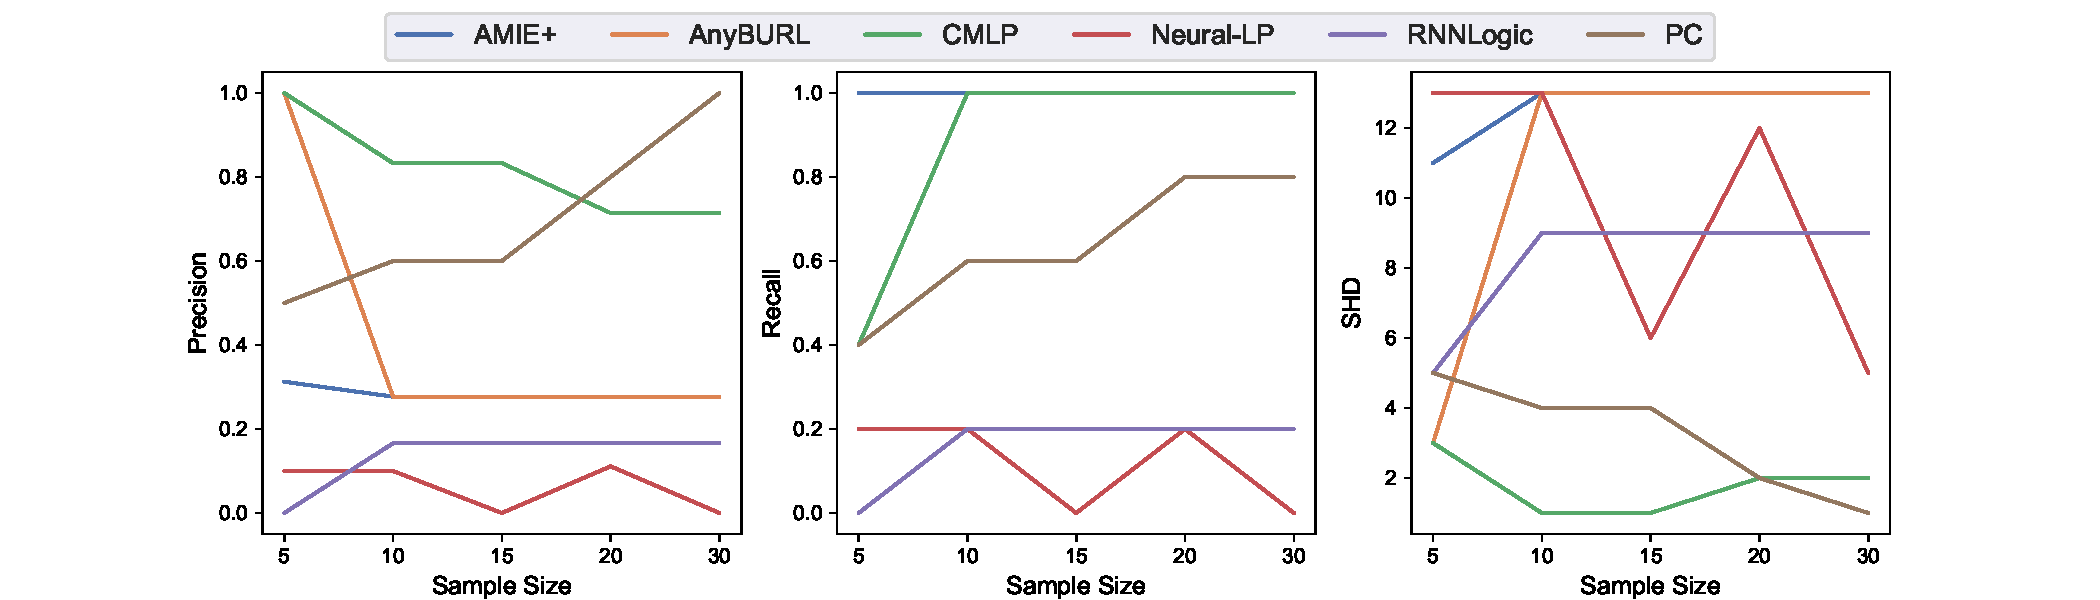
\includegraphics[trim=3cm 0cm 3cm 0cm, width=\linewidth, height=5cm]{figures/allin.pdf}
%     \caption{Precision, recall and SHD results on simulation datasets with differnet sample size. }
%     \label{fig:sim-graph}
% \end{figure*}
\noindent
\textbf{Quality of causal rules from simulations.}
The ground-truth causal graph of KGSs shown in Fig~\ref{fig:simulation}, and
Table~\ref{tab:simulation_rule_quality} shows the accuracy of estimated rules of different methods.
In particular, \dname~ accurately discovers two causal rules in Fig~\ref{fig:simulation} without any redundant rules.
In contrast, correlation-based methods report some non-causal rules.


\begin{table}[t]
\caption{Experimental results on simulation data with $p_{X_1}=0.5$, based on the metrics (precision, recall and SHD), which are commonly used to evaluate the estimated causal graph.}
%\vspace{5pt}
\label{tab:simulation_rule_quality}
\centering
\scalebox{1.2}{
\begin{tabular}{c|c|c|c}
\hline
\textbf{Method} & \textbf{Precision} $\uparrow$ & \textbf{Recall} $\uparrow$ & \textbf{SHD} $\downarrow$ \\
\hline
Neural-LP & 0 & 0& 10 \\
AMIE+ & 0.22 & \textbf{1.0}& 7 \\
RNNLogic & 0.22 & \textbf{1.0}& 7 \\
AnyBURL & 0.25 & \textbf{1.0}& 6 \\
\dname & \textbf{1.0} & \textbf{1.0} & \textbf{0} \\
\hline
\end{tabular}}
\vspace{-4pt}
\end{table}

\begin{table*}[h]
\caption{All rules whose head are $R_3$ and $R_5$, obtained by each algorithm learned on simulated dataset. The strikethroughs indicate the wrong results (there is no entities satisfying the rule).
The rules consistent with the generation process are in bold.
The orange text denotes the weight of each rule with the form max-normalization(original weight)}.

\label{tab:simulation_rule}
\centering
{\tiny
\scalebox{0.75}{
\begin{tabu}{c|l|l|l}
\tabucline[1pt]{-}
\textbf{Method} & \textbf{Rules of $R_3$ with $\mathbf{p_{X_1}=0.5}$} & \textbf{Rules of $R_3$ with $\mathbf{p_{X_1}=0.9}$} & \textbf{Rules of $R_5$}\\
\tabucline[1pt]{-}

\multirow{3}{*}{AMIE+} & \textcolor{orange}{1.00 (0.908)}   $\mathbf{R_3(C_1,C_3) \gets R_1(C_1,C_2), R_2(C_2,C_3)}$  & \textcolor{orange}{1.00 (0.900)}   $\mathbf{R_3(C_1,C_3) \gets R_1(C_1,C_2), R_2(C_2,C_3)}$ & \textcolor{orange}{1.00 (0.898)}   $R_5(C_1,C_3) \gets R_1(C_1,C_2), R_2(C_2,C_3)$\\

& \textcolor{orange}{0.91 (0.829)}   $R_3(C_1,C_3) \gets R_4(C_1,C_3)$ & \textcolor{orange}{0.99 (0.890)}   $R_3(C_1,C_3) \gets R_4(C_1,C_3)$ & \textcolor{orange}{0.99 (0.895)}   $R_5(C_1,C_3) \gets R_3(C_1,C_3)$ \\
&  \textcolor{orange}{0.55 (0.500)}   $R_3(C_1,C_3) \gets R_5(C_1,C_3)$  & \textcolor{orange}{0.91 (0.820)}   $R_3(C_1,C_3) \gets R_5(C_1,C_3)$ & \textcolor{orange}{0.99 (0.894)}   $R_5(C_1,C_3) \gets R_4(C_1,C_3)$\\
\hline
\multirow{3}{*}{AnyBURL}& \textcolor{orange}{1.00 (0.896)} $\mathbf{R_3(C_1,C_3) \gets R_1(C_1,C_2), R_2(C_2,C_3)}$ & \textcolor{orange}{1.00 (0.898)} $R_3(C_1,C_3) \gets R_4(C_1,C_3)$ & \textcolor{orange}{1.00 (0.907)} $R_5(C_1,C_3) \gets R_1(C_1,C_2), R_2(C_2,C_3)$\\
& \textcolor{orange}{0.92 (0.823)} $R_3(C_1,C_3) \gets R_4(C_1,C_3)$ &  \textcolor{orange}{0.99 (0.893)} $\mathbf{R_3(C_1,C_3) \gets R_1(C_1,C_2), R_2(C_2,C_3)}$ & \textcolor{orange}{0.99 (0.902)} $R_5(C_1,C_3) \gets R_3(C_1,C_3)$\\
& \textcolor{orange}{0.56 (0.501)} $R_3(C_1,C_3) \gets R_5(C_1,C_3)$ & \textcolor{orange}{0.91 (0.821)} $R_3(C_1,C_3) \gets R_5(C_1,C_3)$ & \textcolor{orange}{0.99 (0.897)} $R_5(C_1,C_3) \gets R_4(C_1,C_3)$ \\
\hline

\multirow{7}{*}{Neural-LP} & \textcolor{orange}{1.00 (0.318)}  \sout{$R_3(C_1,C_3) \gets R_4(C_1,C_2), R_4(C_2,C_3)$} & \textcolor{orange}{1.00 (0.757)}  \sout{$R_3(C_1,C_3) \gets R_1(C_1,C_2), R_1(C_2,C_3)$}  & \textcolor{orange}{1.00 (0.125)} \sout{$R_5(C_1,C_3) \gets R_4(C_1,C_2),R_3(C_2,C_3)$} \\
& \textcolor{orange}{0.99 (0.316)} \sout{$R_3(C_1,C_3) \gets R_4(C_1,C_2), R_5(C_2,C_3)$} & \textcolor{orange}{0.17 (0.128)} \sout{$R_3(C_1,C_3) \gets R_1(C_1,C_3)$} & \textcolor{orange}{0.78 (0.097)} \sout{$R_5(C_1,C_3) \gets R_3(C_1,C_2),R_3(C_2,C_3)$} \\
& \textcolor{orange}{0.31 (0.100)} \sout{$R_3(C_1,C_3) \gets R_5(C_1,C_2), R_4(C_2,C_3)$} & \textcolor{orange}{0.04 (0.056)} \sout{$R_3(C_1,C_3) \gets R_5(C_2,C_3), R_1(C_1,C_2)$} &\\
& \textcolor{orange}{0.31 (0.099)} \sout{$R_3(C_1,C_3) \gets R_5(C_1,C_2), R_5(C_2,C_3)$} & \textcolor{orange}{0.05 (0.035)} \sout{$R_3(C_1,C_3) \gets R_4(C_2,C_1), R_1(C_3,C_2)$} &\\
& \textcolor{orange}{0.23 (0.073)} $R_3(C_1,C_3) \gets R_4(C_1,C_3)$ & \textcolor{orange}{0.03 (0.025)} $\mathbf{R_3(C_1,C_3) \gets R_1(C_1,C_2), R_2(C_2,C_3)}$\\
& \textcolor{orange}{0.09 (0.028)} \sout{$R_3(C_1,C_3) \gets R_4(C_1,C_2), R_4(C_2,C_3)$} & \\
& \textcolor{orange}{0.07 (0.023)} $R_3(C_1,C_3) \gets R_5(C_1,C_3)$ &\\
\hline

\multirow{3}{*}{RNNLogic} & \textcolor{orange}{1.00 (0.076)}   $\mathbf{R_3(C_1,C_3) \gets R_1(C_1,C_2), R_2(C_2,C_3)}$  & \textcolor{orange}{1.00 (0.071
)}   $\mathbf{R_3(C_1,C_3) \gets R_1(C_1,C_2), R_2(C_2,C_3)}$ & \textcolor{orange}{1.00 (0.220)}   $R_5(C_1,C_3) \gets R_3(C_1,C_3)$\\

& \textcolor{orange}{0.58 (0.044)}   $R_3(C_1,C_3) \gets R_4(C_1,C_3)$ & \textcolor{orange}{0.49 (0.035)}   $R_3(C_1,C_3) \gets R_4(C_1,C_3)$ & \textcolor{orange}{0.28 (0.060)}   $R_5(C_1,C_3) \gets R_4(C_1,C_3)$ \\
&  \textcolor{orange}{0.13 (0.010)}   $R_3(C_1,C_3) \gets R_5(C_1,C_3)$  & \textcolor{orange}{0.14 (0.010)}   $R_3(C_1,C_3) \gets R_5(C_1,C_3)$ & \textcolor{orange}{0.20 (0.045)}   $R_5(C_1,C_3) \gets R_1(C_1,C_2), R_2(C_2,C_3)$\\
\hline


{\dname} & \textcolor{orange}{1.00 (122.797)} $\mathbf{R_3(C_1,C_3) \gets R_1(C_1,C_2), R_2(C_2,C_3)}$ & \textcolor{orange}{1.00 (20.061)} $\mathbf{R_3(C_1,C_3) \gets R_1(C_1,C_2), R_2(C_2,C_3)}$ & -\\

\tabucline[1pt]{-}
\end{tabu}}
}
\end{table*}

\noindent
\textbf{Interpretability of causal rules}
% For rules from the simulation, we analyze all methods' results, whose heads are $R_5$ and $R_6$, and $R_9$ and the results are shown in Table~\ref{tab:simulation_rule} .
% % The rules follow the causal mechanism are in bold.
% There is only one causal rule for $R_5$, which is $R_5(C_1,C_2) \gets R_1(C_1,C_3), R_2(C_3,C_2)$.
% AMIE+, AnyBURL, and \dname~find this causal rule.
% Besides this causal rule, the results of AMIE+ and AnyBURL also include other rules, such as $R_5(C_1,C_2) \gets R_6(C_1,C_2)$ and $R_5(C_1,C_2) \gets R_9(C_1,C_3)$.
% % Especially, for AMIE+ and AnyBURL, note that the weights of $R_3(C_1,C_3) \gets R_4(C_1,C_3)$ are very close to the weights of $R_3(C_1,C_3) \gets R_1(C_1,C_2)$, $ R_2(C_2,C_3)$.
% % It means the algorithms think these two rules have the similar interpretability for the head relation $R_3$.
% % With the change of root node $X_1$'s distribution(from $p_{X_1}=0.5$ to $p_{X_1}=0.9$), AnyBURL even report the higher weight for the rule $R_3(C_1,C_3) \gets R_5(C_1,C_3)$.
% % According to the generation mechanism, the existence of $R_3$ between entities $e_i$ and $e_j$ is independent with whether there is $R_4$ and $R_5$ between $e_i$ and $e_j$.
% % AMIE+ and AnyBURL still return these association rules with high weights, because they only consider whether $R_3$ and $R_4$ co-occur frequently, but not the reason of the co-occurrence.
% The end-to-end deep-model based method(Neural-LP and RNNLogic) fail to discover any correct rules for $R_5$.
Moreover, for the simulation dataset, we analyze all methods' results, whose heads are $R_3$ and $R_5$, and the results are shown in Table~\ref{tab:simulation_rule} (We omit results of $R_4$, since $R_3$ and $R_4$ are symmetric in the causal graph).
The rules follow the causal mechanism are in bold.
There is only one causal rule for $R_3$, which is $R_3(C_1,C_3) \gets R_1(C_1,C_2), R_2(C_2,C_3)$.
AMIE+, AnyBURL, RNNLogic and \dname~find this causal rule.
Besides this causal rule, the results of AMIE+, RNNLogic and AnyBURL also include other rules, such as $R_3(C_1,C_3) \gets R_4(C_1,C_3)$ and $R_3(C_1,C_3) \gets R_5(C_1,C_3)$.
Especially, for those three methods, note that the weights of $R_3(C_1,C_3) \gets R_4(C_1,C_3)$ are very close to the weights of $R_3(C_1,C_3) \gets R_1(C_1,C_2)$, $ R_2(C_2,C_3)$.
It means the algorithms think these two rules have the similar interpretability for the head relation $R_3$.
With the change of root node $X_1$'s distribution(from $p_{X_1}=0.5$ to $p_{X_1}=0.9$), AnyBURL even report the higher weight for the rule $R_3(C_1,C_3) \gets R_5(C_1,C_3)$.
According to the generation mechanism, the existence of $R_3$ between entities $e_i$ and $e_j$ is independent with whether there is $R_4$ and $R_5$ between $e_i$ and $e_j$.
AMIE+, AnyBURL and RNNLogic still return these association rules with high weights, because they only consider whether $R_3$ and $R_4$ co-occur frequently, but not the reason of the co-occurrence.
The end-to-end completion-oriented method, Neural-LP, also return some wrong results, such as the top 1 rule $R_3(C_1,C_3) \gets R_4(C_1,C_2), R_4(C_2,C_3)$, which can not be satisfied by any entities in KG.
The results in~\cite{sadeghian2019drum} show the same phenomenon.
The intermediate results of the completion-oriented method is incomprehensible sometimes.


Furthermore, We sort the rules generated by each algorithm based on their assigned weights and show the five top rules from Douban and Hetionet in Tab.~\ref{tab:rules_recom_result} and Tab.~\ref{tab:rule_hetionet}, respectively.
The results in Tab.~\ref{tab:rules_recom_result} suggests that the ratings for the target movie are highly related to other movies which share the same staff, such as writer, actors, director, etc.
According to the rating results, \dname~ finds a strong causal relationship between the rating of the movie and its editor than other pairs.
The top rules generated by AMIE+ and AnyBURL focus on other shared staffs, but the shared staff has different roles in the target movie and the movie in path.
Those rules of AMIE+ and AnyBURL are hard to be satisfied for most queries.
% By contrast, our mined rules suggest the ratings are determined by the subjective opinions of the users, while the mined rules from other algorithms, including AnyBURL, present the ratings are depended on others related events.
It is worth noting that RNNlogic report the `fan' rules  will impact the users' rating, but \dname~ excludes this kind of rules.
Our results suggest the working ability of the movie's stuff ({\it e.g.} actor or writer) should be the root cause of the users' rate, instead of the followers of the stuff.
From the rules from Hetionet, we can see
% Similar to the results on simulation dataset,
the learned rules are broadly divided into two classes, those in which the target drug and disease are connected by therapeutic information about the similar disease and drug, and those in which the target drug and disease are connected by commonly associated genes.
Further, we find that the rules mined by AnyBURL also contain rules for reasoning through shared side effects.



% Logically incorrect rules are highlighted by italic-red. This experiment shows two of the three top ranked rules generated by Neural LP are incorrect (for both head predicates wif e and son
\begin{table*}[t]
\centering
\caption{Top 5 Rules to infer HighRate(User, Movie) given by the methods. The strikethroughs indicate the wrong results (there is no entities satisfying the rule).
}
\label{tab:rules_recom_result}
\vspace{-1pt}
{\tiny
\begin{tabular}{c|l}
\hline
\textbf{Method} & \multicolumn{1}{c}{\textbf{ Top rules to infer HighRate(User, Movie)}} \\
\hline

\multirow{5}{*}{AMIE+} &
\textcolor{orange}{1.00 (0.565)} HighRate(User,Movie) $\gets$ HighRate(User,Movie1), Writer(Person,Movie1),Director(Person,Movie)\\
& \textcolor{orange}{0.98 (0.556)} HighRate(User,Movie) $\gets$ HighRate(User,Movie1), Director(Person,Movie1), Writer(Person,Movie)\\
& \textcolor{orange}{0.87 (0.489)} HighRate(User,Movie) $\gets$ HighRate(User,Movie1), Writer(Person,Movie1), Actress(Person,Movie)\\
& \textcolor{orange}{0.74 (0.417)} HighRate(User,Movie) $\gets$ HighRate(User,Movie1), Director(Person,Movie1), Actor(Person,Movie)\\
& \textcolor{orange}{0.72 (0.405)} HighRate(User,Movie) $\gets$ HighRate(User,Movie1), Actress(Person,Movie1), Writer(Person,Movie)\\
\hline

\multirow{5}{*}{AnyBURL} &
\textcolor{orange}{1.00 (0.400)} HighRate(User,Movie) $\gets$ HighRate(User,Movie1), Composer(Person,Movie1), Actor(Person,Movie)\\
& \textcolor{orange}{0.99(0.397)} HighRate(User,Movie) $\gets$ HighRate(User,Movie1), Producer(Person,Movie1), Director(Person,Movie)\\
& \textcolor{orange}{0.97 (0.386)} HighRate(User,Movie) $\gets$ HighRate(User,Movie1), Director(Person,Movie1), Actress(Person,Movie)\\
& \textcolor{orange}{0.89 (0.355)} HighRate(User,Movie) $\gets$ HighRate(User,Movie1), Writer(Person,Movie1), Actress(Person,Movie)\\
& \textcolor{orange}{0.85 (0.340)} HighRate(User,Movie) $\gets$ HighRate(User,Movie1), Editor(Person,Movie1), Editor(Person,Movie)\\
\hline



\multirow{2}{*}{Neural-LP}
& \textcolor{orange}{1.00 (0.120)} HighRate(User,Movie) $\gets$ HighRate(User,Movie1), HighRate(User1,Movie1), HighRate(User1,Movie)\\
& \textcolor{orange}{0.28 (0.034)} HighRate(User,Movie) $\gets$ HighRate(User,Movie1), MovieType(Movie1,Type), MovieType(Movie,Type)\\
\hline


\multirow{5}{*}{RNNLogic} &
\textcolor{orange}{1.00 (0.011)} HighRate(User,Movie) $\gets$ Fan(User,Person),Editor(Person,Movie)\\
&\textcolor{orange}{0.45 (0.005)} HighRate(User,Movie) $\gets$ Fan(User,Person),Actor(Person,Movie)\\
&\textcolor{orange}{0.36 (0.004)} HighRate(User,Movie) $\gets$ Fan(User,Person),Director(Person,Movie)\\
&\textcolor{orange}{0.36 (0.004)} HighRate(User,Movie) $\gets$ Fan(User,Person),Writer(Person,Movie)\\
&\textcolor{orange}{0.36 (0.004)} HighRate(User,Movie) $\gets$ Fan(User,Person),Composer(Person,Movie)\\
\hline

\multirow{5}{*}{\dname} &
\textcolor{orange}{1.00 (0.034)} HighRate(User,Movie) $\gets$ HighRate(User,Movie1), Editor(Person,Movie1), Editor(Person,Movie)\\

& \textcolor{orange}{0.12 (0.004)} HighRate(User,Movie1) $\gets$ HighRate(User,Movie1),Cinematographer(Person,Movie),Cinematographer(Person,Movie)
\\
& \textcolor{orange}{0.06 (0.002)} HighRate(User,Movie1) $\gets$ HighRate(User,Movie1),Writer(Person,Movie),Writer(Person,Movie)\\
& \textcolor{orange}{0.06 (0.002)} HighRate(User,Movie1) $\gets$ HighRate(User,Movie1),Actress(Person,Movie),Actress(Person,Movie)\\
& \textcolor{orange}{0.03 (0.001)} HighRate(User,Movie1) $\gets$ HighRate(User,Movie1),Director(Person,Movie),Actor(Person,Movie)\\
\hline
\end{tabular}
}
\end{table*}


\begin{table*}
\centering
\caption{Top 5 Rules to infer Treats(Compound, Disease) given by the methods. For brevity, we use `C' and `D' for compound and disease, respectively.}
\label{tab:rule_hetionet}
{\tiny
\begin{tabular}{c|l}
    \hline
    \textbf{Method} & \multicolumn{1}{c}{\textbf{ Top rules to infer Treats(Compound, Disease)}} \\ \hline
    \multirow{5}{*}{AMIE+} &
\textcolor{orange}{1.00 (0.393)}
Treats(C, D) $\gets$ Resembles(C,C1), Treats(C1, D)
    \\
& \textcolor{orange}{0.82 (0.322)}
Treats(C, D) $\gets$ Resembles(C1,C),Treats(C1, D)
\\
& \textcolor{orange}{0.42 (0.167)} Treats(C, D) $\gets$ Downregulates(C,Gene1), Associates(D,Gene1)
\\
& \textcolor{orange}{0.38 (0.151)} Treats(C, D) $\gets$ Downregulates(C,Gene1), Upregulates(D,Gene1)
 \\
& \textcolor{orange}{0.37 (0.144)} Treats(C, D) $\gets$ Binds(C,Gene1), Upregulates(D,Gene1)
\\


\hline
\multirow{5}{*}{AnyBURL} & \textcolor{orange}{1.00 (0.319)}
Treats(C, D) $\gets$ Includes(PharmacologicClass1,C),Includes(PharmacologicClass1,C1),Treats(C1, D)
 \\
& \textcolor{orange}{0.60 (0.192)}
Treats(C, D) $\gets$ Resembles(C1,C),Treats(C1, D)
 \\
& \textcolor{orange}{0.52 (0.166)}
Treats(C, D) $\gets$ Resembles(C1,C),Resembles(C1,C2),Treats(C2, D)
 \\
& \textcolor{orange}{0.31 (0.098)}
Treats(C, D) $\gets$ Resembles(C1,C),Resembles(C2,C1),Treats(C2, D)
 \\
& \textcolor{orange}{0.24 (0.077)}
Treats(C, D) $\gets$ Treats(C, D1), Resembles(D1,D)
 \\ \hline


\multirow{1}{*}{Neural-LP} &
\textcolor{orange}{1.00 (0.659)}
Treats(C, D) $\gets$ Treats(C, D1), Treats(C1, D1),Treats(C1, D)
\\ \hline



\multirow{2}{*}{RNNLogic} &
\textcolor{orange}{1.00 (0.00007)}
Treats(C, D) $\gets$ Resembles(C, C1),Treats(C1, D)
 \\
& \textcolor{orange}{1.00 (0.00007)}

Treats(C, D) $\gets$ Resembles(C, C1),
Resembles(C1, C2),Treats(C2, D)
\\ \hline


\multirow{5}{*}{\dname} &
\textcolor{orange}{1.00 (269.00))}
Treats(C, D) $\gets$ Treats(C, D1),Resembles(D1, D2),Resembles(D, D2)
 \\
    & \textcolor{orange}{0.85 (229.32))}
Treats(C, D) $\gets$ Includes(PharmacologicClass1, C),Includes(PharmacologicClass1, C1),Treats(C1, D)

\\
    & \textcolor{orange}{0.83 (224.37))}
Treats(C, D) $\gets$
Treats(C, D1),Resembles(D2, D1),Resembles(D2, D)
\\
    & \textcolor{orange}{0.58 (155.18))}
Treats(C, D) $\gets$ Treats(C, D1),Treats(C1, D1),Treats(C1, D)


\\
    & \textcolor{orange}{0.10 (26.52))}
 Treats(C, D) $\gets$
 Treats(C, D1),
 Resembles(D2,D1),
 Resembles(D,D1)

    \\ \hline

\end{tabular}
}
\end{table*}


% \begin{table*}
% \caption{Top Rules to infer $User\stackrel{Rate}{\longrightarrow}Movie$ given by the methods.}
% \label{tab:rule_douban}
% \begin{tabular}{c|l}
%     \hline
%     \textbf{Method} & \multicolumn{1}{c}{\textbf{ Top rules to infer $User\stackrel{Rate}{\longrightarrow}Movie$}} \\ \hline
%     \multirow{3}{*}{AMIE+} &
%     1. $User\stackrel{Fan}{\longrightarrow}Person\stackrel{Director}{\longrightarrow}Movie$ \\
%     & 2. $User\stackrel{Fan}{\longrightarrow}Person\stackrel{Writer}{\longrightarrow}Movie$ \\
%     & 3. $User\stackrel{Rate}{\longrightarrow}Movie1\stackrel{Director}{\longleftarrow}Person\stackrel{Director}{\longrightarrow}Movie$ \\ \hline
%     \multirow{3}{*}{AnyBURL} &  1. $User\stackrel{Rate}{\longrightarrow}Movie1\stackrel{Wish}{\longleftarrow}User1\stackrel{Rate}{\longrightarrow}Movie$ \\
%     & 2. $User\stackrel{Rate}{\longrightarrow}Movie1\stackrel{Director}{\longleftarrow}Person\stackrel{Actor}{\longrightarrow}Movie$ \\
%     & 3. $User\stackrel{Rate}{\longrightarrow}Movie1\stackrel{Producer}{\longleftarrow}Person\stackrel{Actor}{\longrightarrow}Movie$ \\ \hline
%     \multirow{3}{*}{Neural-LP} & 1. $User\stackrel{Rate}{\longrightarrow}Movie1\stackrel{Rate}{\longleftarrow}User1\stackrel{Rate}{\longrightarrow}Movie$ \\
%     & 2. $User\stackrel{Rate}{\longrightarrow}Movie1\stackrel{titleType}{\longleftarrow}MovieType\stackrel{titleType}{\longrightarrow}Movie$ \\
%     & 3. $User\stackrel{Wish}{\longrightarrow}Movie1\stackrel{archivesound}{\longleftarrow}Person\stackrel{archivesound}{\longrightarrow}Movie$ \\ \hline
%     \multirow{3}{*}{RNNLogic} & 1. $User\stackrel{Fan}{\longrightarrow}Person\stackrel{Actor}{\longrightarrow}Movie$ \\
%     & 2. $User\stackrel{Fan}{\longrightarrow}Person\stackrel{Director}{\longrightarrow}Movie$ \\
%     & 3. $User\stackrel{Fan}{\longrightarrow}Person\stackrel{Writer}{\longrightarrow}Movie$ \\ \hline
%     \multirow{3}{*}{\dname} & 1. $User\stackrel{Rate}{\longrightarrow}Movie1\stackrel{Writer}{\longleftarrow}Person\stackrel{Writer}{\longrightarrow}Movie$ \\
%     & 2. $User\stackrel{Rate}{\longrightarrow}Movie1\stackrel{Actress}{\longleftarrow}Person\stackrel{Actress}{\longrightarrow}Movie$ \\
%     & 3.$User\stackrel{Rate}{\longrightarrow}Movie1\stackrel{Director}{\longleftarrow}Person\stackrel{Actor}{\longrightarrow}Movie$ \\ \hline
% \end{tabular}
% \end{table*}

% \begin{table*}[t]
% \centering
% \caption{Top 3 Rules of HighRate given by the methods.The strikethroughs indicate the wrong results (there is no entities satisfying the rule).
% The orange text denotes the weight of each rule with the form max-normalization(original weight)}
% \label{tab:rules_recom_result}
% \vspace{-1pt}
% \begin{tabular}{c|l}
% \hline
% \textbf{Method} & \multicolumn{1}{c}{\textbf{Rules of HighRate}} \\
% \hline
% \multirow{3}{*}{Neural-LP} &
% \textcolor{orange}{1.00 (0.636)} \sout{HighRate(User,Movie) $\gets$ Saw(User1,Movie), Saw(User2,User1)}\\
%  &    \textcolor{orange}{0.50 (0.320)} \sout{HighRate(User,Movie) $\gets$ Saw(User1,Movie), Saw(User2,User1),Saw(User,User2)} \\
%   &  \textcolor{orange}{0.02(0.011)}  HighRate(User,Movie) $\gets$ Saw(User, Movie)\\
% \hline
% \multirow{3}{*}{AMIE+} &
% \textcolor{orange}{1.00 (0.662)} HighRate(User,Movie) $\gets$ Fan(User, Person), Director(Person,Movie) \\
% & \textcolor{orange}{0.99 (0.658)} HighRate(User,Movie) $\gets$ Fan(User, Person), Writer(Person,Movie) \\
% & \textcolor{orange}{0.85 (0.565)} HighRate(User,Movie) $\gets$ HighRate(User,Movie1), Writer(Person,Movie1),Director(Person,Movie)\\
% \hline
% \multirow{5}{*}{AnyBURL} &
% \textcolor{orange}{1.00 (0.286)} HighRate(User,Movie) $\gets$ HighRate(User,Movie1), Wish(User1,Movie1),HighRate(User1,Movie) \\
% & \textcolor{orange}{0.97 (0.276)} HighRate(User,Movie) $\gets$ HighRate(User,Movie1), Director(Person,Movie1),Actor(Person,Movie)
% \\
% & \textcolor{orange}{0.97 (0.276)} HighRate(User,Movie) $\gets$ HighRate(User,Movie1), Producer(Person,Movie1),Actor(Person,Movie)\\
% & $\dots$ \\
% & \textcolor{orange}{0.983 (0.236)} HighRate(User,Movie) $\gets$ Fan(User,Person), Director(Person,Movie) \\
% \hline
% \multirow{3}{*}{RNNLogic} &
% \textcolor{orange}{1.00 (0.0048)} HighRate(User,Movie) $\gets$ Fan(User,Person), Actor(Person,Movie) \\
% & \textcolor{orange}{0.875 (0.0042)} HighRate(User,Movie) $\gets$ Fan(User,Person), Director(Person,Movie) \\
% & \textcolor{orange}{0.85 (0.0041)} HighRate(User,Movie) $\gets$ Fan(User,Person), Writer(Person,Movie) \\

% \hline
% \multirow{3}{*}{\dname} &
% \textcolor{orange}{1.00 (0.035)} HighRate(User,Movie) $\gets$ HighRate(User,Movie1),Writer(Person,Movie1),Writer(Person,Movie) \\
% & \textcolor{orange}{0.06 (0.002)} HighRate(User,Movie1) $\gets$ HighRate(User,Movie1),Actress(Person,Movie),Actress(Person,Movie)
% \\
% & \textcolor{orange}{0.06 (0.002)} HighRate(User,Movie1) $\gets$ HighRate(User,Movie1),Director(Person,Movie),Actor(Person,Movie)\\
% \hline
% \end{tabular}
% \end{table*}

% We conducted an experimental study in which we investigated the performance of the learned causal rules in two aspects: the explainability to the KG and the usefulness for downstream task, such as link prediction.
% Our main goal is to provide insight into
% \begin{itemize}
%     \item the explainability of the learned causal rules to the KG.
%     \item the effectiveness of the learned causal rules or downstream task, such as link prediction.
%     \item the empirical conclusions for the hyper-parameters and alternative algorithms in our framework.
% \end{itemize}
% Furthermore, we briefly summarize the experiment designs to achieve the above-mentioned the goal under the available resources.

% Goal 1 	$\Rightarrow$ We use the simulation KG to quantitatively evaluate the learned causal rules from KG, since the causal relationships are inaccessible for real dataset\footnote{This is the most commonly used way for the evaluation of the causal discovery methods in both relational and propositional data\cite{zheng2018dags, lee2016learning}}.
% Meanwhile, the case study for real data will be introduced to qualitatively discuss the quality of mined rules.

% Goal 2 	$\Rightarrow$ 
%!TEX root = ../main.tex
\section{Related Works}
\label{sec:related}

\stitle{Retrieval Augmented Generation Question Answering.}
%
Large languaga models sometimes generate factually incorrect or misleading information, often due to a lack of real-time knowledge or limited access to external facts beyond their training data.
RAG-based Question Answering addresses this by integrating external knowledge retrieval into the generation process. By retrieving relevant document chunks through semantic search, RAG ensures that the model’s responses are grounded in accurate, real-world information, effectively reducing the likelihood of hallucinations.
Early approaches focused on jointly training the retriever and generator, ensuring that the retrieved content aligned with the generation model’s intent to provide more accurate answers~\cite{izacard2023atlas}. With the success of in-context learning, more recent work has treated the retriever as a separate module, directly providing retrieved information to the model via prompts~\cite{wang2023knowledgptenhancinglargelanguage}.
As retrieval technologies have advanced, RAG-based systems now support multimodal retrieval, enabling answers that draw from diverse data sources~\cite{chen2021open, chen-etal-2022-murag, luo-etal-2023-unifying}. 
%For example, OTT-QA~\cite{chen2021open}  retrieves both tables and text, MuRAG~\cite{chen-etal-2022-murag} integrates text and images, and MMQA~\cite{luo-etal-2023-unifying} combines text, tables, and images to handle complex queries.
% \yang{It's hard for us to compare Symphony with existing systems.}


\stitle{Trustworthiness of Large Language Models.}
%
The trustworthiness of LLMs is essential for their effective deployment in real-world applications. To assess LLM trustworthiness, researchers have proposed various approaches. For example, TrustLLM~\cite{huang2024trustllmtrustworthinesslargelanguage} provides a comprehensive framework for evaluating LLMs across different trust dimensions.
However, evaluating LLM trustworthiness remains challenging, with gaps in holistic assessment approaches. Some studies suggest that self-evaluation, where LLMs assess their confidence in the generated outputs, can help improve selective generation and mitigate inaccuracies~\cite{Ren2023SelfEvaluationIS}. Additionally, understanding the internal mechanisms of LLMs, such as the use of local intrinsic dimension (LID) for predicting truthfulness, has been proposed as a way to measure model reliability~\cite{Yin2024CharacterizingTI}.
In our work, we aim to improve the trustworthiness of LLMs through post-verification, ensuring that generated outputs are validated against reliable sources after generation to minimize inaccuracies and enhance their overall reliability.
\section{Concluding Remarks}
\label{sec:discussion}
In this paper, we reconcile efficiency and security for uplink communication in Federated Learning. 
We propose to adapt existing compression mechanisms such as scalar quantization and pruning to the secure aggregation protocol by imposing a linearity constraint on the decompression operator. 
Our experiments demonstrate that we can adapt both quantization and pruning mechanisms to obtain a high degree of uplink compression with minimal degradation in performance and higher security guarantees. For achieving the highest rates of compression, we introduce \SecInd, a variant of \SecAgg well-suited for TEE-based implementation that supports product quantization while maintaining a high security bar. 
%We plan to extend our work to other federated learning scenarios, such as asynchronous FL, and further investigate the interaction of compression and privacy.
%\section{Extensions} 
As mentioned in Section~\ref{sec:intro}, we {may want } both \SecAgg and Differential Privacy~\citep{abadi2016deep} to realize the full promise of FL as a privacy-enhancing technology. 
While our primary focus is on enabling efficient and secure uplink communication, we emphasize that the proposed approaches are compatible with user-level DP. 
For instance, {at the cost of increasing the complexity of the trusted computing base}, DP noise can be added natively by the TEE with our modified random pruning or scalar quantization approaches. 
For PQ  and \SecInd, {we can have the TEE to add noise in the assignment space (\ie outputting a noisy histogram), or to map the histogram to the codeword space and add noise there.
Each option offers a different tradeoff between privacy, trust, and accuracy; we leave detailed evaluation to future work.}




%\modif{\textbf{Compatibility with DP.} 
%\sout{it would require, however, to transfer the aggregation to TEE or to design a DP mechanism in the assignment space, since DP noise must be added by the TEE and not by the server.}}

%\modif{\textbf{Efficiency and Privacy.}} A separate line of work {aims} to combine communication efficiency and privacy. 
%For instance, \cite{triastcyn2021dprec} develop a method that unifies compressed communication and DP (where integration with \SecAgg is left as an open problem), while \cite{chaudhuri2022privacyaware} design a privacy-aware scalar compression mechanism within the \emph{local} differential privacy model.

%\graham{\sout{
%\modif{\textbf{Broader Social Impact. }} In this work, we propose to enhance the privacy of individuals who may contribute to training ML models and simultaneously enable more individuals to participate in private training, who might otherwise have been excluded due to resource constraints. }}
% Indeed, Federated Learning could enable a malicious server to access individual model updates that can leak personal information. Hence, we propose a secure way to communicate the individual model updates.

% - Generic and less data-dependent codebook
% - Model compression 
% - Compression and DP
% - Error correction

% There are multiple extensions of PQ, such as having multiple codebooks per matrix  (which increases the cost of storing the codebooks) or performing the assignments with other norms than the $L_2$ norm.



% As a side note, \cite{jia2022federated} propose to perform domain adaptation by fine-tuning a small fraction of the model parameters, which is naturally compatible with Secure Aggregation, but requires to start from a pretrained model. 





%%
%% The next two lines define the bibliography style to be used, and
%% the bibliography file.

\begin{thebibliography}{10}

\bibitem{Bonawitz2017PracticalSA}
K.~Bonawitz, V.~Ivanov, B.~Kreuter, A.~Marcedone, H.~McMahan, S.~Patel,
  D.~Ramage, A.~Segal, and K.~Seth.
\newblock Practical secure aggregation for privacy-preserving machine learning.
\newblock {\em CCS}, 2017.

\bibitem{chai2020secure}
D.~Chai, L.~Wang, K.~Chen, and Q.~Yang.
\newblock Secure federated matrix factorization.
\newblock {\em IEEE Intelligent Systems}, 2020.

\bibitem{ganti2011mobile}
R.~K. Ganti, F.~Ye, and H.~Lei.
\newblock Mobile crowdsensing: current state and future challenges.
\newblock {\em IEEE Communications Magazine}, 49(11):32--39, 2011.

\bibitem{han2021hidden}
X.~Han, L.~Wang, and W.~Fan.
\newblock Is hidden safe? location protection against machine-learning
  prediction attacks in social networks.
\newblock {\em MIS Quarterly}, 45(2):821--858, 2021.

\bibitem{konevcny2016federated}
J.~Kone{\v{c}}n{\`y}, H.~B. McMahan, F.~X. Yu, P.~Richt{\'a}rik, A.~T. Suresh,
  and D.~Bacon.
\newblock Federated learning: Strategies for improving communication
  efficiency.
\newblock {\em arXiv:1610.05492}, 2016.

\bibitem{li2014the}
H.~{Li}, B.~{Zhao}, and A.~{Fuxman}.
\newblock The wisdom of minority: discovering and targeting the right group of
  workers for crowdsourcing.
\newblock In {\em WWW}, pages 165--176, 2014.

\bibitem{li2016survey}
Y.~Li, J.~Gao, C.~Meng, Q.~Li, L.~Su, B.~Zhao, W.~Fan, and J.~Han.
\newblock A survey on truth discovery.
\newblock {\em SIGKDD Explor. Newsl.}, 17(2):1–16, Feb. 2016.

\bibitem{Li2018AnET}
Y.~Li, C.~Miao, L.~Su, J.~Gao, Q.~Li, B.~Ding, Z.~Qin, and K.~Ren.
\newblock An efficient two-layer mechanism for privacy-preserving truth
  discovery.
\newblock {\em KDD}, 2018.

\bibitem{Li2020TowardsDP}
Y.~Li, H.~Xiao, Z.~Qin, C.~Miao, L.~Su, J.~Gao, K.~Ren, and B.~Ding.
\newblock Towards differentially private truth discovery for crowd sensing
  systems.
\newblock {\em ICDCS}, pages 1156--1166, 2020.

\bibitem{liu2020secure}
Y.~{Liu}, Y.~{Kang}, C.~{Xing}, T.~{Chen}, and Q.~{Yang}.
\newblock A secure federated transfer learning framework.
\newblock {\em IEEE Intelligent Systems}, 35(4):70--82, 2020.

\bibitem{ma2014opportunities}
H.~Ma, D.~Zhao, and P.~Yuan.
\newblock Opportunities in mobile crowd sensing.
\newblock {\em IEEE Communications Magazine}, 52(8):29--35, 2014.

\bibitem{meng2015truth}
C.~Meng, W.~Jiang, Y.~Li, J.~Gao, L.~Su, H.~Ding, and Y.~Cheng.
\newblock Truth discovery on crowd sensing of correlated entities.
\newblock In {\em Proceedings of the 13th ACM Conference on Embedded Networked
  Sensor Systems}, pages 169--182, 2015.

\bibitem{Miao2015CloudEnabledPT}
C.~Miao, W.~Jiang, L.~Su, Y.~Li, S.~Guo, Z.~Qin, H.~Xiao, J.~Gao, and K.~Ren.
\newblock Cloud-enabled privacy-preserving truth discovery in crowd sensing
  systems.
\newblock In {\em SenSys}, 2015.

\bibitem{Miao2019PrivacyPreservingTD}
C.~Miao, W.~Jiang, L.~Su, Y.~Li, S.~Guo, Z.~Qin, H.~Xiao, J.~Gao, and K.~Ren.
\newblock Privacy-preserving truth discovery in crowd sensing systems.
\newblock {\em ACM Transactions on Sensor Networks}, 15:1 -- 32, 2019.

\bibitem{Miao2017ALP}
C.~Miao, L.~Su, W.~Jiang, Y.~Li, and M.~Tian.
\newblock A lightweight privacy-preserving truth discovery framework for mobile
  crowd sensing systems.
\newblock {\em INFOCOM}, pages 1--9, 2017.

\bibitem{ouyang2015truth}
R.~W. Ouyang, M.~Srivastava, A.~Toniolo, and T.~J. Norman.
\newblock Truth discovery in crowdsourced detection of spatial events.
\newblock {\em IEEE transactions on knowledge and data engineering},
  28(4):1047--1060, 2015.

\bibitem{Peng2018DataQG}
D.~Peng, F.~Wu, and G.~Chen.
\newblock Data quality guided incentive mechanism design for crowdsensing.
\newblock {\em IEEE Transactions on Mobile Computing}, 17:307--319, 2018.

\bibitem{epflmobility}
M.~Piorkowski, N.~Sarafijanovic-Djukic, and M.~Grossglauser.
\newblock {CRAWDAD} dataset epfl/mobility (v. 2009-02-24).
\newblock Downloaded from \url{https://crawdad.org/epfl/mobility/20090224},
  Feb. 2009.

\bibitem{Primault2019TheLR}
V.~Primault, A.~Boutet, S.~B. Mokhtar, and L.~Brunie.
\newblock The long road to computational location privacy: A survey.
\newblock {\em IEEE Communications Surveys \& Tutorials}, 21:2772--2793, 2019.

\bibitem{Reddy2010ExaminingMF}
S.~Reddy, D.~Estrin, M.~Hansen, and M.~Srivastava.
\newblock Examining micro-payments for participatory sensing data collections.
\newblock {\em UbiComp}, 2010.

\bibitem{shamir1979share}
A.~Shamir.
\newblock How to share a secret.
\newblock {\em Communications of the ACM}, 22(11):612--613, 1979.

\bibitem{tang2011secure}
C.~Tang, G.~Shi, and Z.~Yao.
\newblock Secure multi-party computation protocol for sequencing problem.
\newblock {\em SCIENTIA SINICA Informationis}, 41(7):789--797, 2011.

\bibitem{Tang2018NonInteractivePT}
X.~Tang, C.~Wang, X.~Yuan, and Q.~Wang.
\newblock Non-interactive privacy-preserving truth discovery in crowd sensing
  applications.
\newblock {\em INFOCOM}, pages 1988--1996, 2018.

\bibitem{Wang2014SurrogateMS}
D.~Wang, T.~Abdelzaher, and L.~M. Kaplan.
\newblock Surrogate mobile sensing.
\newblock {\em IEEE Communications Magazine}, 52:36--41, 2014.

\bibitem{wang2013credibility}
D.~Wang, L.~Kaplan, T.~Abdelzaher, and C.~C. Aggarwal.
\newblock On credibility estimation tradeoffs in assured social sensing.
\newblock {\em IEEE Journal on Selected Areas in Communications},
  31(6):1026--1037, 2013.

\bibitem{wang2012truth}
D.~Wang, L.~Kaplan, H.~Le, and T.~Abdelzaher.
\newblock On truth discovery in social sensing: A maximum likelihood estimation
  approach.
\newblock In {\em IPSN}, pages 233--244, 2012.

\bibitem{Wang2017LocationPT}
L.~Wang, D.~Yang, X.~Han, T.~Wang, D.~Zhang, and X.~Ma.
\newblock Location privacy-preserving task allocation for mobile crowdsensing
  with differential geo-obfuscation.
\newblock {\em WWW}, 2017.

\bibitem{Wang2019MobileCT}
L.~Wang, D.~Yang, X.~Han, D.~Zhang, and X.~Ma.
\newblock Mobile crowdsourcing task allocation with differential-and-distortion
  geo-obfuscation.
\newblock {\em IEEE Transactions on Dependable and Secure Computing},
  18:967--981, 2021.

\bibitem{Wang2020SparseMC}
L.~Wang, D.~Zhang, D.~Yang, B.~Y. Lim, X.~Han, and X.~Ma.
\newblock Sparse mobile crowdsensing with differential and distortion location
  privacy.
\newblock {\em IEEE Transactions on Information Forensics and Security},
  15:2735--2749, 2020.

\bibitem{wang2016differential}
L.~Wang, D.~Zhang, D.~Yang, B.~Y. Lim, and X.~Ma.
\newblock Differential location privacy for sparse mobile crowdsensing.
\newblock In {\em ICDM}, pages 1257--1262. IEEE, 2016.

\bibitem{Wang2021AST}
T.~Wang, C.~Lv, C.~Wang, F.~Chen, and Y.~Luo.
\newblock A secure truth discovery for data aggregation in mobile crowd
  sensing.
\newblock {\em Secur. Commun. Networks}, 2021:2296386:1--2296386:15, 2021.

\bibitem{Wang2019PersonalizedPT}
Z.~Wang, J.~Hu, R.~Lv, J.~Wei, Q.~Wang, D.~Yang, and H.~Qi.
\newblock Personalized privacy-preserving task allocation for mobile
  crowdsensing.
\newblock {\em IEEE Transactions on Mobile Computing}, 18:1330--1341, 2019.

\bibitem{Whitehill2009WhoseVS}
J.~Whitehill, P.~Ruvolo, T.~Wu, J.~Bergsma, and J.~Movellan.
\newblock Whose vote should count more: Optimal integration of labels from
  labelers of unknown expertise.
\newblock In {\em NeurIPS}, 2009.

\bibitem{Xu2019EfficientAP}
G.~Xu, H.~Li, S.~Liu, M.~Wen, and R.~Lu.
\newblock Efficient and privacy-preserving truth discovery in mobile crowd
  sensing systems.
\newblock {\em IEEE Transactions on Vehicular Technology}, 68:3854--3865, 2019.

\bibitem{yang2019federated}
Q.~Yang, Y.~Liu, T.~Chen, and Y.~Tong.
\newblock Federated machine learning: Concept and applications.
\newblock {\em ACM Transactions on Intelligent Systems and Technology},
  10(2):12, 2019.

\bibitem{yin2008truth}
X.~Yin, J.~Han, and S.~Y. Philip.
\newblock Truth discovery with multiple conflicting information providers on
  the web.
\newblock {\em IEEE Transactions on Knowledge and Data Engineering},
  20(6):796--808, 2008.

\bibitem{ZHANG2020101848}
C.~Zhang, C.~Xu, L.~Zhu, Y.~Li, C.~Zhang, and H.~Wu.
\newblock An efficient and privacy-preserving truth discovery scheme in
  crowdsensing applications.
\newblock {\em Computers \& Security}, 97:101848, 2020.

\bibitem{Zhang2021ReliableAP}
C.~Zhang, L.~Zhu, C.~Xu, X.~Liu, and K.~Sharif.
\newblock Reliable and privacy-preserving truth discovery for mobile
  crowdsensing systems.
\newblock {\em IEEE Transactions on Dependable and Secure Computing},
  18:1245--1260, 2021.

\bibitem{zhang20144w1h}
D.~Zhang, L.~Wang, H.~Xiong, and B.~Guo.
\newblock 4w1h in mobile crowd sensing.
\newblock {\em IEEE Communications Magazine}, 52(8):42--48, 2014.

\bibitem{Zheng2018LearningTT}
Y.~Zheng, H.~Duan, and C.~Wang.
\newblock Learning the truth privately and confidently: Encrypted
  confidence-aware truth discovery in mobile crowdsensing.
\newblock {\em IEEE Transactions on Information Forensics and Security},
  13:2475--2489, 2018.

\bibitem{Zheng2020PrivacyAwareAE}
Y.~Zheng, H.~Duan, X.~Yuan, and C.~Wang.
\newblock Privacy-aware and efficient mobile crowdsensing with truth discovery.
\newblock {\em IEEE Transactions on Dependable and Secure Computing},
  17:121--133, 2020.

\end{thebibliography}



\appendix

\section{Datasets for FEL}
\label{sec:datasets}
In this section we would like to provide more details about our experiments. We first provide details about each dataset that was used. We then provide details about the model architectures that we used for each dataset.  


\subsection{Production Dataset}
Production dataset is an internal dataset that captures whether a user installs a mobile application after being shown a relevant advertisement item. A few hundred features are used as an input (the exact number cannot be disclosed) to predict a binary label (install/not-install). All the input features are public. For training, we use advertisement data from a random sample of 35 million users over a period of one month. Randomly selected 15 million users from the following week were used for testing.  

%\subsection{Open-Source Datasets}

\subsection{Taobao CTR Dataset}
The Taobao dataset contains 26 million interactions (click/non-click when an Ad was shown) between 1.14 million users and 847 thousand items across an 8-day period. 
The dataset uses 9 user features (e.g., gender or occupation), 6 item features (e.g., price or brand), and two contextual features (e.g., the day of week), which we assume to be all public to the service provider. 

In the Taobao CTR dataset, 16 out of the 17 features are sparse, with a categorical value encoding instead of a continuous, floating point value.
%
While server-based recommendation models use large embedding tables to convert these sparse features into a floating point embedding~\cite{din, dlrm, wideanddeep}, training such embedding tables on device is complicated because of the large memory capacity requirement (e.g., in the order of GB to TB~\cite{zhao2020distributed,acun:2021:understandingtraining,wilkening:2021:recssd,lui:2021:capacity}) and can leak private information more easily through gradients~\cite{alibaba_fl}. %significantly~\cite{zhang2021wide}.
Thus, we assume an architecture where embedding tables are pre-trained with opt-in users and are hosted on the server, while the rest of the model is trained with FEL using sparse features translated through the pre-trained tables. We randomly selected 10\% of the users as opt-in.

Note that our setup cannot achieve the accuracy that can be reached when we fully train the embedding tables, as we pre-train the embedding table and fix their weight during FL.
However, our setup represents a practical FL setup where training embedding tables on-device is prohibitive, due to client resource limitations~\cite{nguyen2021federated} and privacy concerns~\cite{alibaba_fl}.




\subsection{CelebA Smile Prediction Dataset}
While FEL is originally designed for recommendation and ranking tasks, we study its generality to non-recommendation models with CelebFaces Attributes Dataset (CelebA)~\cite{liu2015deep}. CelebA consists of $200,288$ images belonging to $9,343$ unique celebrities. Each image has 40 binary facial attribute annotations (e.g., bald, long hair, attractive, etc) and covers large pose variations and backgrounds.
We defined distinguishing between smiling/non-smiling images as our target task.

The Taobao dataset contains 26 million interactions (click/non-click when an Ad was shown) between 1.14 million users and 847 thousand items across an 8-day period. 
The dataset uses 9 user features (e.g., gender or occupation), 6 item features (e.g., price or brand), and two contextual features (e.g., the day of week), which we assume to be all public to the service provider. The details on how we preprocess the  dataset can be found in the appendix. 




\subsection{Model Architectures}
{\bf Production/Taobao Dataset:}
For recommendation datasets (production/Taobao CTR), we use a model that consists of 3 fully-connected hidden layers. The number of units at each hidden layer is decreasing exponentially with a parameter K. For instance, if $K=4$ and the input layer has 512 features, our neural network would have  $[512, 128, 32, 8, 1]$ neurons. For each dataset, we tune K to obtain a resulting model of approximately $10$MB. By doing so, it allows us to train a neural network even on older, low-tier devices with more limited memory capacity. ReLu is used as an activation function after each layer apart from the last one, where Sigmoid and binary cross-entropy was used.

For both datasets, we use synchronous FL with FedAvg~\cite{mcmahan2017learning}. We used the following hyperparameters for the Taobao dataset from an extensive hyperparameter search: client batch size of 32, 5 local epochs, 4096 clients per round, and a learning rate of 0.579 with SGD. Clients are selected at random and each only participates once (1 global epoch). The production dataset used similar hyperparameters.

For Taobao dataset's server-side pre-trained embedding table, we use an embedding dimension of 32, and train it with the 10\% opt-in users for 1 epoch using AdaGrad optimizer with learning rate of 0.01.

{\bf CelebA Dataset:}
For CelebA, we follow the setup of prior work~\cite{nguyen2021federated} and use a four layer CNN with dropout rate of 0.1, stride of 1, and padding of 2. We preprocess all images in train/validation/test sets; each image is resized and cropped to 32$\times$32 pixels, then normalized by 0.5 mean and 0.5 standard deviation. We use asynchronous FL with a client batch size of 32 samples, 1 local epoch, 30 global epochs, and a learning rate of 0.899 with SGD.

\section{Evaluation Methodology}
\label{sec:appendix-b}
Our evaluation aims to answer the following questions:

\begin{itemize}
    \item Can FEL improve the model prediction quality over vanilla FL? [Section~\ref{sec:prediction-quality}]
    \item How do different ensemble aggregation methods affect the model accuracy? [Section~\ref{sec:prediction-quality}]
    \item How do different clustering methods affect the model accuracy? [Section~\ref{sec:prediction-quality-clustering}]
    \item How does FEL affect privacy compared to vanilla FL? [Section~\ref{sec:privacy-eval}]
\end{itemize}

To answer these questions we used the three datasets presented in Section~\ref{sec:datasets}. To study recommendation and ranking tasks, we used a production dataset and an open-source, Taobao's Click-Through-Rate (CTR) prediction dataset~\cite{li2021novel}.
To study the effect of FEL on non-recommendation use-cases, we additionally studied the LEAF CelebA Smile Prediction dataset~\cite{liu2015deep}. More details about these datasets and their associated model architecture can be found in Section~\ref{sec:datasets}.


Both the FL baseline and the FEL leaf models used the same set of hyperparameters. 
The FL baseline is trained using all the available client data. In FEL, the client data is clustered, and one leaf model is trained for each cluster. We vary the number of clusters from 3--10 and evaluate different clustering methods.
When training the over-arch NN layer, a small subset of opt-in users is used.


\begin{table}
\small
\centering
\caption{\label{tab:clusterconfig} Explanation of different cluster methods in Figure~\ref{fig:eval0} (right).}
\begin{tabular}{|l||l|l|c|}
\hline
Dataset & Config & Feature & \# clusters \\ \hline\hline
\multirow{4}{*}{Production} & Clustering 1 & Age & 5\\
 & Clustering 2 & App & 5\\
 & Clustering 3 & Location & 4\\
 & Clustering 4 & Click ratio & 10\\\hline
\multirow{3}{*}{Taobao~\cite{taobao}} & Clustering 1 & Age & 7\\
 & Clustering 2 & Consumption & 4\\
 & Clustering 3 & City level & 5\\\hline
\multirow{3}{*}{CelebA~\cite{liu2015deep}} & Clustering 1 & \# Attributes & 3\\
 & Clustering 2 & K-means & 3\\
 & Clustering 3 & K-means & 5\\\hline
\end{tabular}\\
\end{table}



\end{document}
\endinput
%%
%% End of file `sample-sigconf.tex'.
